\chapter{Réalisation}

\section*{Introduction}
Dans ce chapitre, nous débutons par décrire l'environnement de travail en mentionnant les technologies et les outils que nous avons utilisés. Ensuite, nous présentons l'architecture de déploiement de notre solution. Enfin, nous concluons en présentant les différentes interfaces Homme/Machine que nous avons développées.

%% ============================================================
%%  4.1  DIAGRAMME DE DÉPLOIEMENT
%% ============================================================
\section{Diagramme de déploiement}

Dans ce qui suit, nous décrivons l'architecture logicielle de notre plateforme CRM à travers le diagramme de déploiement présenté ci-dessous par la figure~\ref{fig:deploiement}.

\begin{figure}[H]
    \centering
    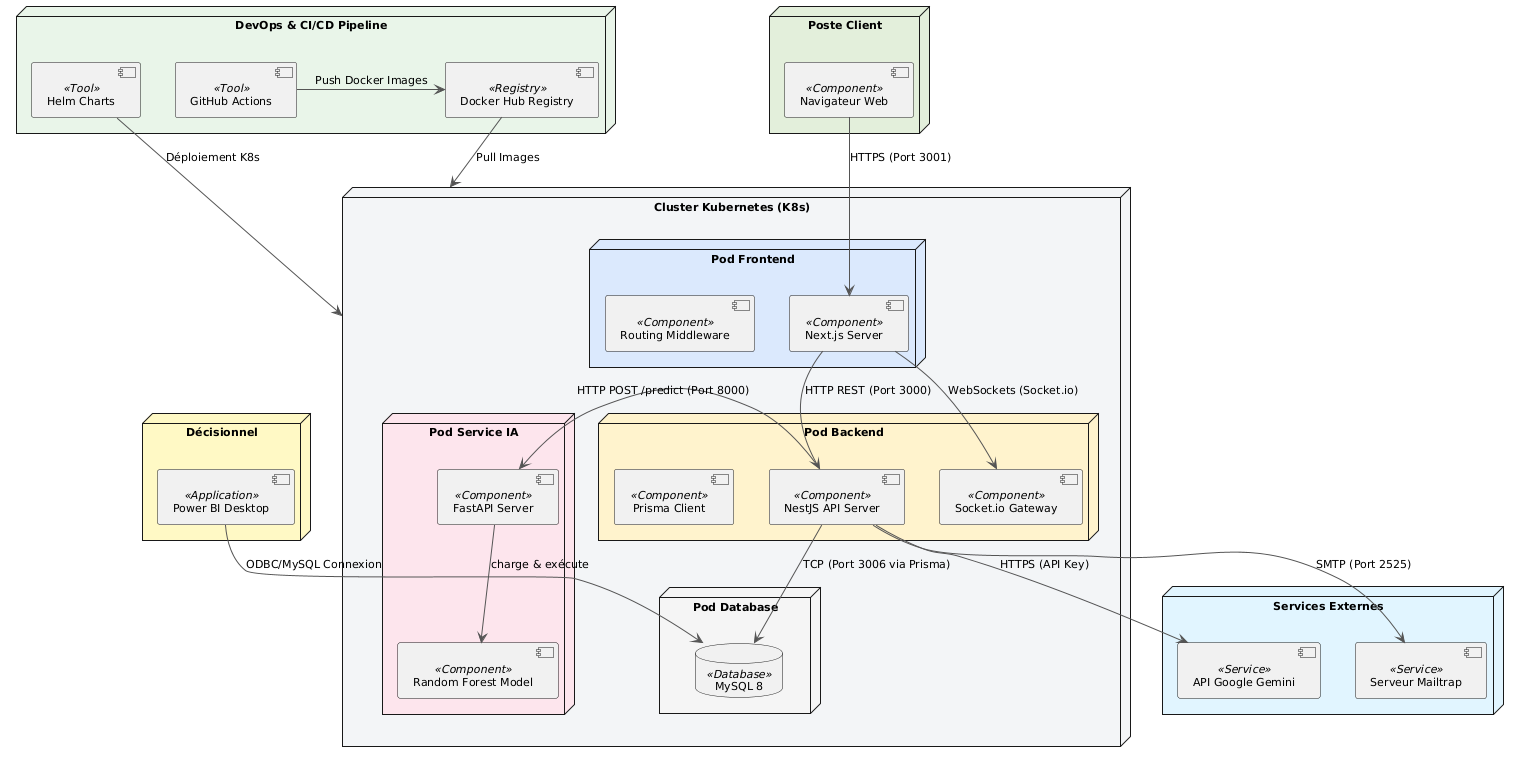
\includegraphics[width=\textwidth,height=0.82\textheight,keepaspectratio]{images/diagramme_deploiement.png}
    \caption{Diagramme de déploiement}
    \label{fig:deploiement}
\end{figure}

Le tableau~\ref{tab:composants} décrit les différents composants matériels et logiciels de notre système.

\begin{table}[H]
\centering
\renewcommand{\arraystretch}{1.4}
\begin{tabular}{|p{3.5cm}|p{10cm}|}
\hline
\textbf{Nom} & \textbf{Description} \\
\hline
Next.js (Frontend) & Framework React pour le rendu côté serveur et la génération de pages statiques, servant l'interface utilisateur de la plateforme CRM. \\
\hline
NestJS (Backend) & Framework Node.js progressif pour la construction d'API REST efficaces et évolutives, gérant la logique métier et l'accès aux données. \\
\hline
FastAPI (AI Agent) & Framework Python haute performance pour la construction du microservice d'intelligence artificielle dédié au scoring des leads. \\
\hline
MySQL & Système de gestion de base de données relationnelle utilisé pour le stockage persistant de toutes les données de l'application. \\
\hline
Prisma ORM & Outil de mapping objet-relationnel (ORM) moderne pour Node.js et TypeScript, facilitant les interactions avec la base de données MySQL. \\
\hline
Docker & Plateforme de conteneurisation permettant d'encapsuler chaque service dans un conteneur isolé et reproductible. \\
\hline
Docker Compose & Outil d'orchestration multi-conteneurs permettant de définir et gérer l'ensemble des services de la plateforme. \\
\hline
Kubernetes (K8s) & Système d'orchestration de conteneurs pour le déploiement, la mise à l'échelle et la gestion automatisée des applications conteneurisées. \\
\hline
Helm & Gestionnaire de packages pour Kubernetes, simplifiant le déploiement et la gestion des charts applicatifs. \\
\hline
GitHub Actions & Service d'intégration et de déploiement continus (CI/CD) permettant d'automatiser le pipeline de build, test et déploiement. \\
\hline
Docker Hub & Registre d'images Docker utilisé pour stocker et distribuer les images conteneurisées de nos services. \\
\hline
Socket.io & Bibliothèque de communication en temps réel basée sur les WebSockets, utilisée pour le chat et les notifications en temps réel. \\
\hline
Power BI & Outil de Business Intelligence de Microsoft utilisé pour la création de tableaux de bord analytiques avancés. \\
\hline
Gemini AI & API d'intelligence artificielle générative de Google, utilisée pour la génération d'e-mails personnalisés et pour propulser le chatbot intelligent avec approche RAG. \\
\hline
\end{tabular}
\caption{Description des composants matériels et logiciels du système}
\label{tab:composants}
\end{table}

%% ============================================================
%%  4.2  STYLE ARCHITECTURAL
%% ============================================================
\section{Le style architectural}

\subsection{Partie front-end}

\subsubsection{Architecture MVC avec Next.js}

L'architecture de notre application front-end repose sur le pattern \textbf{MVC} (Model-View-Controller) adapté au framework Next.js à travers l'App Router. Cette architecture favorise une séparation claire des responsabilités, permettant une maintenance plus aisée et facilitant les tests unitaires.

\begin{itemize}
    \item \textbf{Modèle (Model)} : Le modèle est géré par les hooks personnalisés et le store Zustand. Il représente l'état de l'application et la logique d'accès aux données via les appels API vers le backend NestJS.
    \item \textbf{Vue (View)} : La vue est constituée des composants React (TSX) utilisant Radix UI pour les composants d'interface, TailwindCSS pour le style et Framer Motion pour les animations. Elle est responsable de l'affichage et de la gestion des interactions utilisateur.
    \item \textbf{Contrôleur (Controller)} : Le contrôleur est implémenté à travers les Server Components et les handlers d'événements dans les pages Next.js. Il orchestre la communication entre le modèle et la vue, gère la navigation via le middleware d'authentification et le routage basé sur les rôles (Admin/Rep).
\end{itemize}

\begin{figure}[H]
    \centering
    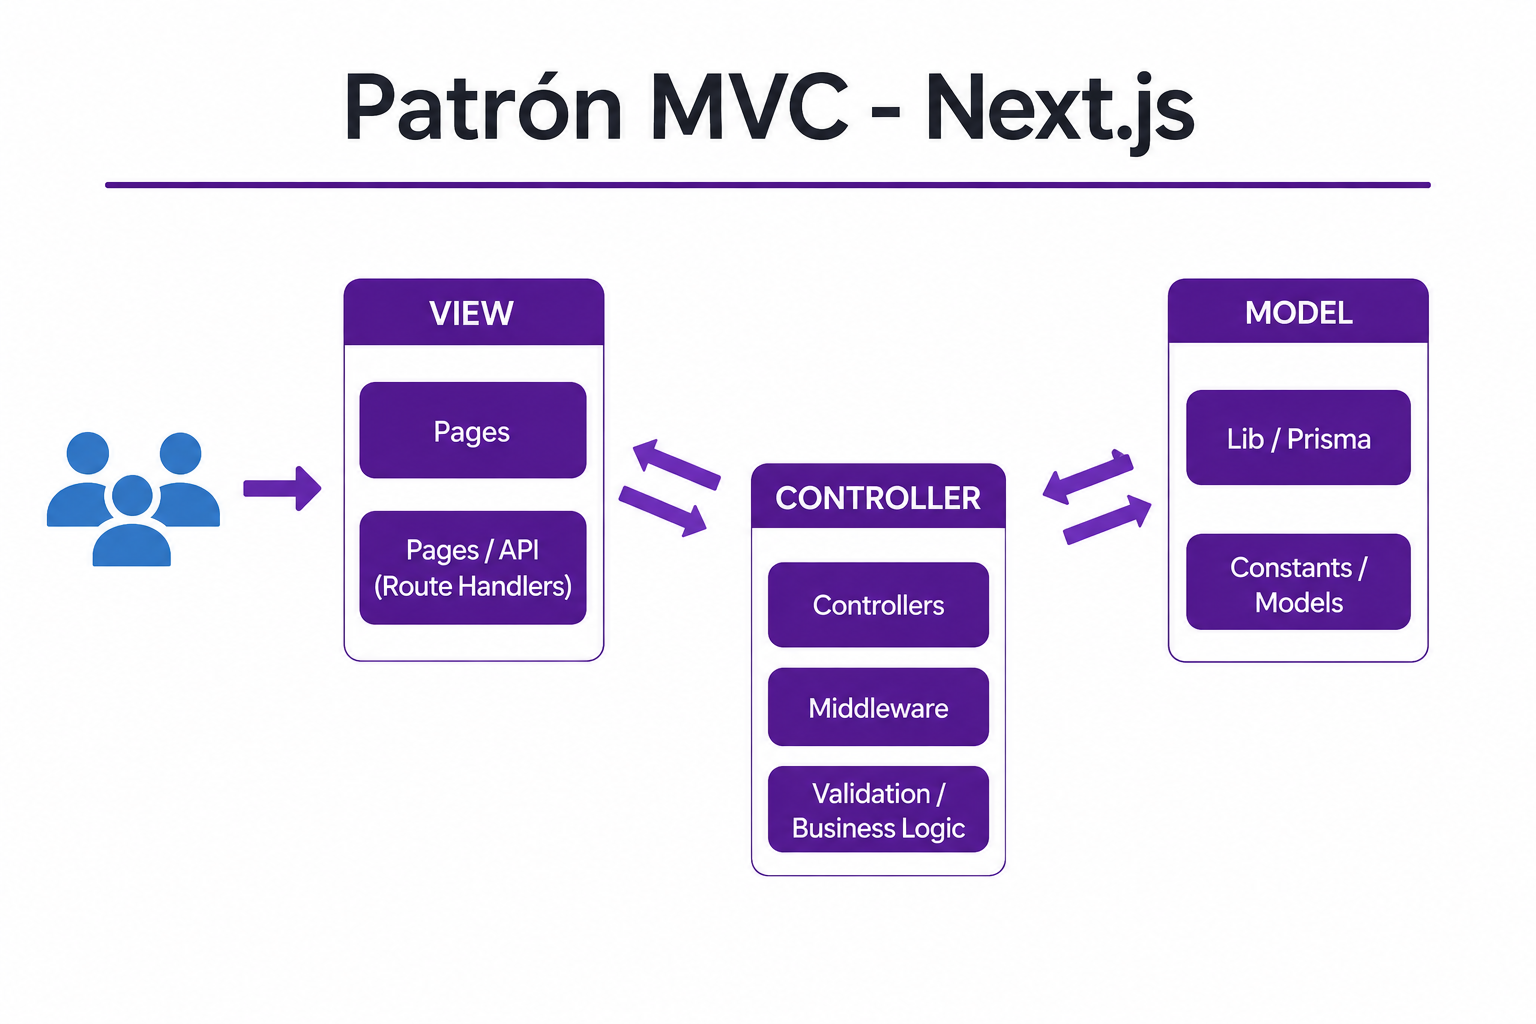
\includegraphics[width=\textwidth,height=0.82\textheight,keepaspectratio]{images/architecture_mvc_nextjs.png}
    \caption{Architecture MVC du front-end}
    \label{fig:mvc}
\end{figure}

\subsubsection{Diagramme de composants front-end}

Ce diagramme présente une vue d'ensemble de notre application web, illustrant les différents modules développés : le module d'authentification, les tableaux de bord Admin et Sales Rep, les modules de gestion (Leads, Contacts, Companies, Pipeline, Tickets), le module de chat en temps réel, ainsi que les intégrations avec l'API Gemini et le service de scoring IA.

\begin{figure}[H]
    \centering
    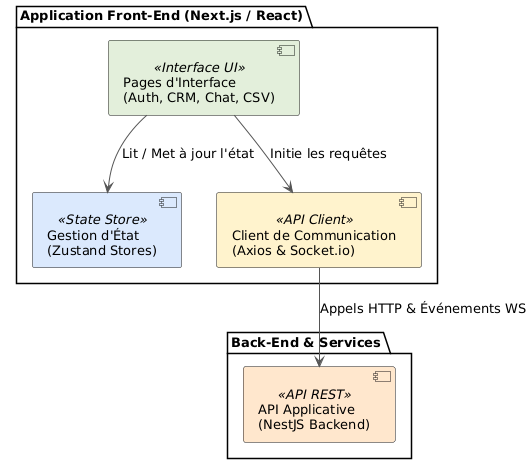
\includegraphics[width=\textwidth,height=0.82\textheight,keepaspectratio]{images/diagramme_composants_frontend.png}
    \caption{Diagramme de composants de l'application web}
    \label{fig:composants-frontend}
\end{figure}

\subsection{Partie back-end}

\subsubsection{Architecture Modulaire NestJS}

L'architecture back-end repose sur le framework \textbf{NestJS}, qui adopte une approche modulaire inspirée d'Angular. Chaque fonctionnalité métier est encapsulée dans un module indépendant contenant ses propres contrôleurs, services et DTOs (Data Transfer Objects). Cette architecture favorise :

\begin{itemize}
    \item La \textbf{séparation des préoccupations} : chaque module gère un domaine métier spécifique (leads, contacts, deals, tickets, etc.).
    \item La \textbf{réutilisabilité} : les services peuvent être injectés dans d'autres modules via le système d'injection de dépendances.
    \item La \textbf{testabilité} : chaque service peut être testé unitairement de manière isolée grâce à l'injection de dépendances.
    \item La \textbf{scalabilité} : l'ajout de nouvelles fonctionnalités se fait par la création de nouveaux modules sans impacter les existants.
\end{itemize}

\begin{figure}[H]
    \centering
    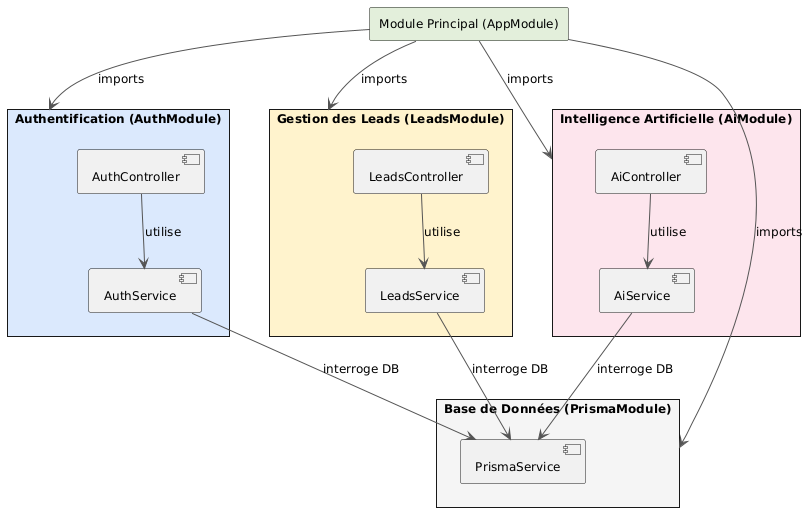
\includegraphics[width=\textwidth,height=0.82\textheight,keepaspectratio]{images/architecture_backend.png}
    \caption{Architecture modulaire du back-end NestJS}
    \label{fig:archi-backend}
\end{figure}

\subsubsection{Architecture Microservices -- Agent IA}

Le service de \textbf{Lead Scoring} est conçu comme un microservice indépendant basé sur \textbf{FastAPI} (Python). Ce service implémente un modèle de Machine Learning (\textit{Random Forest Classifier}) entraîné sur un dataset de scoring de leads. Il communique avec le backend NestJS via des appels HTTP REST.

L'architecture microservices intègre deux avantages majeurs :
\begin{itemize}
    \item \textbf{Indépendance technologique} : le service IA utilise Python et scikit-learn, tandis que le backend principal utilise Node.js/TypeScript, chaque service exploitant les meilleures technologies pour son domaine.
    \item \textbf{Scalabilité indépendante} : le service de scoring peut être mis à l'échelle indépendamment du backend principal en fonction de la charge de prédiction.
\end{itemize}

\begin{figure}[H]
    \centering
    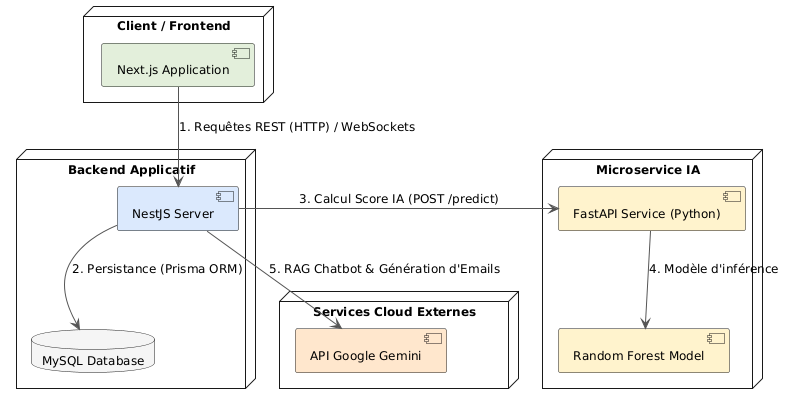
\includegraphics[width=\textwidth,height=0.82\textheight,keepaspectratio]{images/architecture_microservices.png}
    \caption{Architecture microservices -- Agent IA de scoring}
    \label{fig:archi-microservices}
\end{figure}

\subsubsection{Diagramme de composants back-end}

% \begin{figure}[H]
%     \centering
%     % \includegraphics[width=\textwidth]{images/diagramme_composants_backend.png}
%     \caption{Diagramme de composants back-end}
%     \label{fig:composants-backend}
% \end{figure}

%% ============================================================
%%  4.3  ENVIRONNEMENT DE DÉVELOPPEMENT
%% ============================================================
\section{Environnement de développement}

Dans cette partie, nous décrivons les différents outils matériels et logiciels utilisés tout au long de la concrétisation de notre solution.

\subsection{Technologies de programmation}

\subsubsection{Node.js}
Node.js est un environnement d'exécution JavaScript construit sur le moteur V8 de Google Chrome. Il dispose de fonctionnalités exceptionnelles qui en font un choix attrayant pour la création d'applications côté serveur, notamment des serveurs web et des services web. Node.js utilise un modèle d'entrées-sorties non bloquant, basé sur les événements, qui le rend léger et efficace, asynchrone par défaut. Dans notre projet, Node.js (version 22) constitue le socle d'exécution de notre backend NestJS et de notre frontend Next.js.
\begin{figure}[H]
    \centering
    
\includegraphics[width=0.6\textwidth,height=0.45\textheight,keepaspectratio]{images/node.png}
    \caption{Node.js}
    \label{fig:node}
\end{figure}

\subsubsection{Python}
Python est un langage de programmation interprété, polyvalent et à typage dynamique. Il est particulièrement prisé dans le domaine de la \textit{data science} et du \textit{machine learning} grâce à son écosystème riche en bibliothèques spécialisées. Dans notre projet, Python est utilisé pour le développement du microservice d'intelligence artificielle de scoring des leads, exploitant les bibliothèques \texttt{scikit-learn}, \texttt{pandas} et \texttt{numpy}.
\begin{figure}[H]
    \centering
    
\includegraphics[width=0.6\textwidth,height=0.45\textheight,keepaspectratio]{images/python.png}
    \caption{Python}
    \label{fig:python1}
\end{figure}

\subsection{Langages de programmation}

\subsubsection{TypeScript}
TypeScript est un langage compilé, fortement typé, orienté objet, conçu par Microsoft. Il représente un sur-ensemble typé de JavaScript, ajoutant le typage statique, les interfaces et les décorateurs. Dans notre projet, TypeScript est utilisé tant côté front-end (Next.js/React) que côté back-end (NestJS), garantissant une cohérence du code et une détection précoce des erreurs à la compilation.
\begin{figure}[H]
    \centering
    
\includegraphics[width=0.45\textwidth,height=0.4\textheight,keepaspectratio]{images/typescipt.png}
    \caption{TypeScript}
    \label{fig:typescript}
\end{figure}

\subsubsection{Python}
Python est utilisé comme langage principal pour le développement du microservice de Lead Scoring basé sur FastAPI. Sa syntaxe concise et ses bibliothèques de \textit{machine learning} (scikit-learn, pandas, numpy) en font le choix idéal pour l'implémentation de notre modèle prédictif \textit{Random Forest Classifier}.
\begin{figure}[H]
    \centering
    
\includegraphics[width=0.6\textwidth,height=0.45\textheight,keepaspectratio]{images/python.png}
    \caption{Python - Microservice IA}
    \label{fig:python2}
\end{figure}

\subsection{Frameworks}

\subsubsection{Next.js}
Next.js (version 16) est un framework React de production développé par Vercel. Il offre le rendu côté serveur (SSR), la génération de sites statiques (SSG), le routage basé sur le système de fichiers via l'App Router, ainsi qu'un système de middleware intégré. Dans notre projet, Next.js gère l'intégralité de l'interface utilisateur avec un système de routage basé sur les rôles (Admin et Sales Rep).
\begin{figure}[H]
    \centering
    
\includegraphics[width=0.6\textwidth,height=0.45\textheight,keepaspectratio]{images/next.png}
    \caption{Next.js}
    \label{fig:next}
\end{figure}

\subsubsection{NestJS}
NestJS (version 10) est un framework Node.js progressif pour la construction d'applications côté serveur efficaces et évolutives. Inspiré d'Angular, il adopte une architecture modulaire avec injection de dépendances, décorateurs et une structure opinionnée. Notre backend NestJS expose des API REST documentées via Swagger et gère l'authentification JWT, la communication WebSocket et l'envoi d'e-mails.
\begin{figure}[H]
    \centering
    
\includegraphics[width=0.6\textwidth,height=0.45\textheight,keepaspectratio]{images/nest.png}
    \caption{Nest.js}
    \label{fig:nest}
\end{figure}

\subsubsection{FastAPI}
FastAPI est un framework web Python moderne et haute performance pour la construction d'API. Il exploite les annotations de type Python pour la validation automatique des données et la génération de documentation OpenAPI. Dans notre projet, FastAPI héberge le modèle de \textit{machine learning} de scoring des leads et expose les endpoints de prédiction.
\begin{figure}[H]
    \centering
    
\includegraphics[width=0.6\textwidth,height=0.45\textheight,keepaspectratio]{images/fast.png}
    \caption{FastAPI}
    \label{fig:fastapi}
\end{figure}

\subsection{Base de données}

\subsubsection{Système de gestion de base de données}
\textbf{MySQL 8} : Tout au long du développement de notre application, nous avons utilisé MySQL 8 comme système de gestion de base de données relationnelle. MySQL offre une fiabilité, des performances et une facilité d'utilisation reconnues. Il gère l'ensemble des données de notre CRM : utilisateurs, leads, contacts, entreprises, pipelines, deals, tâches, tickets, e-mails, messages de chat et notifications.
\begin{figure}[H]
    \centering
    
\includegraphics[width=0.6\textwidth,height=0.45\textheight,keepaspectratio]{images/sql.png}
    \caption{MySQL}
    \label{fig:mysql}
\end{figure}

\subsubsection{ORM -- Prisma}
\textbf{Prisma} est un ORM (Object-Relational Mapping) moderne pour Node.js et TypeScript. Il fournit un client de base de données type-safe auto-généré, un système de migrations déclaratives et un langage de schéma intuitif. Prisma simplifie considérablement les interactions avec MySQL en offrant une API fluide et en garantissant la sécurité des types à la compilation.
\begin{figure}[H]
    \centering
    
\includegraphics[width=0.45\textwidth,height=0.4\textheight,keepaspectratio]{images/prisma.png}
    \caption{Prisma}
    \label{fig:prisma}
\end{figure}

\subsection{Outils de développement}

\subsubsection{Visual Studio Code}
Visual Studio Code (VS Code) est un éditeur de code source léger mais puissant, développé par Microsoft. Il supporte le débogage, le contrôle Git intégré, la coloration syntaxique, l'auto-complétion intelligente et un écosystème riche en extensions. VS Code est notre IDE principal pour le développement TypeScript (front-end et back-end) et Python (agent IA).
\begin{figure}[H]
    \centering
    
\includegraphics[width=0.45\textwidth,height=0.4\textheight,keepaspectratio]{images/vscode.png}
    \caption{Visual Studio Code}
    \label{fig:vscode}
\end{figure}

\subsubsection{Docker \& Docker Compose}
Docker est une plateforme de conteneurisation permettant de placer nos applications ainsi que leurs dépendances dans des conteneurs indépendants et réutilisables. Docker Compose gère l'ensemble de ces quatre services (MySQL, Backend NestJS, Frontend Next.js, AI Agent FastAPI) avec un fichier de configuration \texttt{docker-compose.yaml}.
\begin{figure}[H]
    \centering
    
\includegraphics[width=0.6\textwidth,height=0.45\textheight,keepaspectratio]{images/docker.png}
    \caption{Docker}
    \label{fig:docker}
\end{figure}

\subsubsection{Kubernetes \& Helm}
Kubernetes est une plate-forme open source d'orchestration de containers qui facilite le déploiement, le scaling et la gestion des applications dans des conteneurs. Helm, qui est un package manager pour Kubernetes, nous donne la possibilité de créer des charts réutilisables pour chaque service de notre plate-forme.
\begin{figure}[H]
    \centering
    
\includegraphics[width=0.6\textwidth,height=0.45\textheight,keepaspectratio]{images/kubernetes.png}
    \caption{Kubernetes and Helm}
    \label{fig:kubernetes}
\end{figure}

\subsubsection{GitHub \& GitHub Actions}
Nous utilisons GitHub comme plateforme pour héberger nos codes sources. GitHub Actions fournit un pipeline CI/CD pour nous avec quatre jobs : build/test des applications, la vérification de la qualité du code par ESLint, la construction de l'image Docker puis sa publication dans Docker Hub, et enfin la modification du tag image des charts Helm.
\begin{figure}[H]
    \centering
    
\includegraphics[width=0.6\textwidth,height=0.45\textheight,keepaspectratio]{images/github.png}
    \caption{GitHub and GitHub Actions}
    \label{fig:github}
\end{figure}

\subsubsection{Postman}
Postman est un outil de test excellent pour l'examen et le test de nos API RESTful. Postman nous offre une interface utilisateur où l'on peut faire nos requêtes HTTP sans avoir besoin de coder pour tester la bonne marche de nos endpoints NestJS et FastAPI.
\begin{figure}[H]
    \centering
    
\includegraphics[width=0.6\textwidth,height=0.45\textheight,keepaspectratio]{images/postman.png}
    \caption{Postman}
    \label{fig:postman}
\end{figure}

\subsubsection{Swagger}
Swagger (à travers le module \texttt{@nestjs/swagger}) fournit une documentation de notre API REST backend en temps réel avec un interface interactif. Cette documentation est accessible depuis le navigateur et elle aide les développeurs à explorer tous les endpoints.
\begin{figure}[H]
    \centering
    
\includegraphics[width=0.45\textwidth,height=0.4\textheight,keepaspectratio]{images/swagger.png}
    \caption{Swagger}
    \label{fig:swagger}
\end{figure}

\subsubsection{Power BI}
Le Power BI est un outil d'analyse d'affaires ou Business Intelligence développé par Microsoft qui est utilisé pour l'analyse interactive via la conception de tableaux de bord. Pour le projet courant, le Power BI est configuré afin d'accéder à notre base de données MySQL et générer des rapports interactifs des données sur nos performances et nos leads.
\begin{figure}[H]
    \centering
    
\includegraphics[width=0.6\textwidth,height=0.45\textheight,keepaspectratio]{images/powerbi.png}
    \caption{Microsoft Power BI}
    \label{fig:powerbi}
\end{figure}

\subsubsection{Draw.io}
Draw.io est un logiciel d'édition de diagramme en ligne totalement gratuit pour créer différents types de diagramme comme le diagramme UML, les diagrammes de séquence, les diagrammes de déploiement et des modèles. Nous avons utilisé Draw.io pour concevoir toutes les figures mentionnées dans ce rapport.
\begin{figure}[H]
    \centering
    
\includegraphics[width=0.6\textwidth,height=0.45\textheight,keepaspectratio]{images/draw.png}
    \caption{Draw.io}
    \label{fig:drawio}
\end{figure}

\subsubsection{Overleaf}
Overleaf est un site collaboratif d'écriture basé sur le logiciel de traitement de texte LaTeX. Il permet à plusieurs personnes de travailler simultanément sur un même document et propose de nombreux modèles de documents déjà prédéfinis. Nous avons utilisé Overleaf pour rédiger ce rapport de PFE.
\begin{figure}[H]
    \centering
    
\includegraphics[width=0.6\textwidth,height=0.45\textheight,keepaspectratio]{images/overleaf.png}
    \caption{Overleaf}
    \label{fig:overleaf}
\end{figure}

%% ============================================================
%%  4.4  PRÉSENTATION DE L'APPLICATION
%% ============================================================
\section{Présentation de l'application}

Dans cette partie, nous donnerons un aperçu des interfaces de notre plateforme CRM développées à travers quelques captures d'écran.

\subsection{Module d'authentification}

\subsubsection{Interface de connexion}
Le module de connexion autorise les utilisateurs à se connecter en utilisant leurs adresses électroniques et mots de passe. La validation des informations est effectuée par JWT (JSON Web Token) et ensuite, ils sont réorientés au tableau de bord qui leur est dédié d'après leur statut qui peut être soit \textbf{Admin} soit \textbf{Rep}.

\begin{figure}[H]
    \centering
    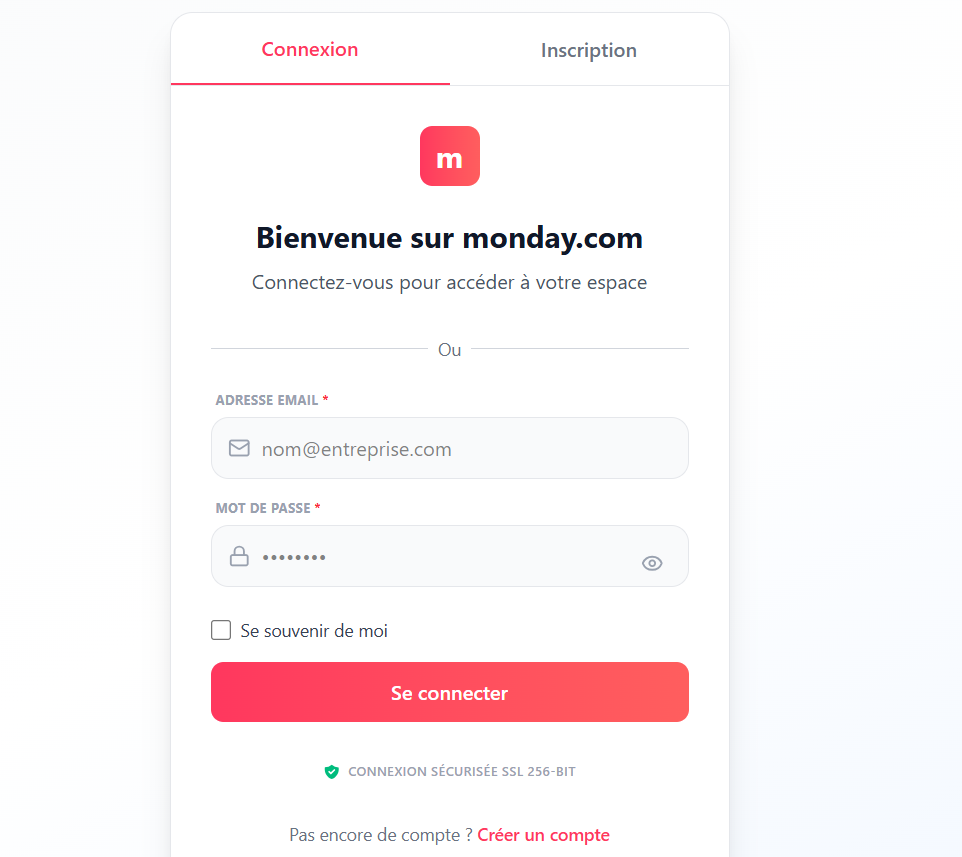
\includegraphics[width=\textwidth,height=0.82\textheight,keepaspectratio]{images/interface_login.png}
    \caption{Interface de connexion}
    \label{fig:login}
\end{figure}

\subsubsection{Interface d'inscription}
The registration interface provides an opportunity for a new user to register by entering his name, email address, password, and company. The role defaults to Sales Representative (Rep).

\begin{figure}[H]
    \centering
    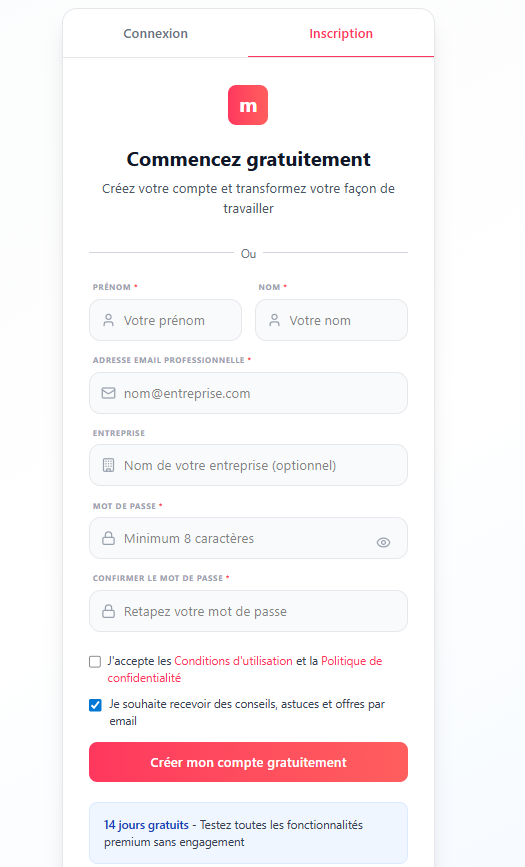
\includegraphics[width=\textwidth,height=0.82\textheight,keepaspectratio]{images/interface_register.png}
    \caption{Interface d'inscription}
    \label{fig:register}
\end{figure}

\subsection{Partie Admin (Sales Manager)}

\subsubsection{Interface tableau de bord Admin}
Après l'authentification, le Sales Manager est automatiquement dirigé vers son dashboard principal. Ce dashboard fournit un aperçu des principaux KPIs qui incluent le nombre total de leads, de contacts, de deals actuels, de taux de conversion, ainsi qu'un diagramme pour analyser l'évolution du chiffre d'affaires et la segmentation des leads selon leurs statuts.

\begin{figure}[H]
    \centering
    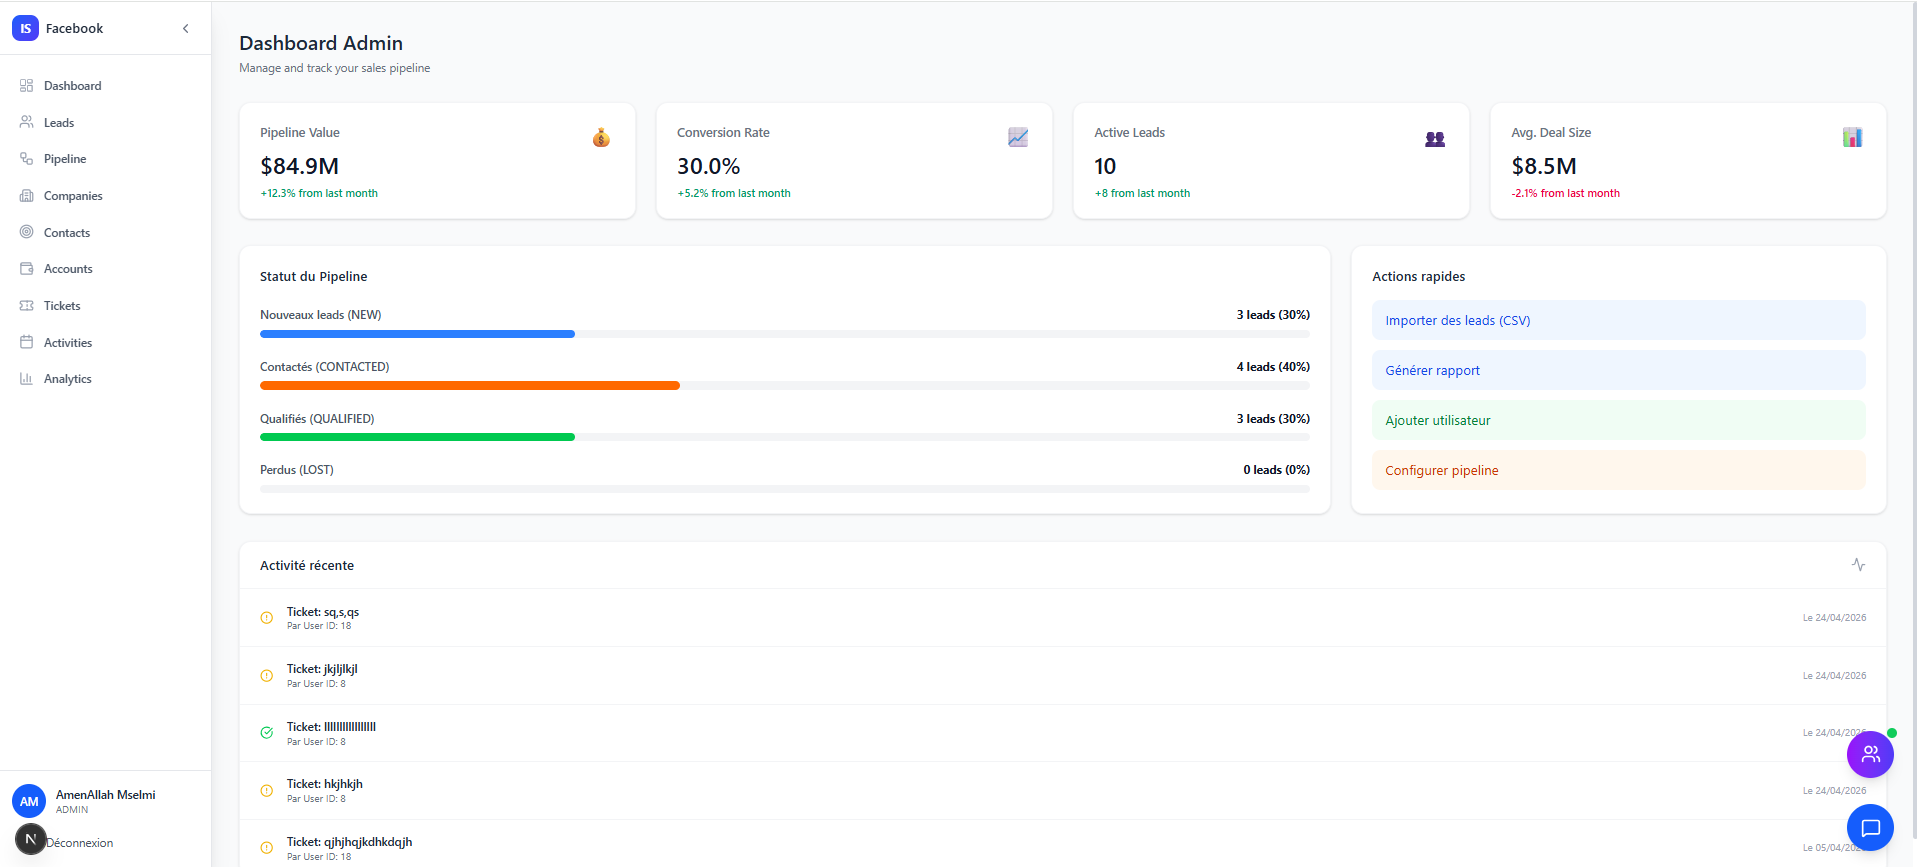
\includegraphics[width=\textwidth,height=0.82\textheight,keepaspectratio]{images/interface_dashboard_admin.png}
    \caption{Interface tableau de bord Admin}
    \label{fig:dashboard-admin}
\end{figure}

\subsubsection{Interface gestion des leads}
Cette interface aide l'administrateur à voir, rechercher, filtrer et gérer tous les leads. Les informations affichées pour chaque lead incluent son nom, email, numéro de téléphone, statut (Nouveau, Contacté, Qualifié, Perdu), valeur du lead et le score de l'IA. En outre, l'administrateur peut accéder aux informations détaillées sur un lead, y compris ses notes, tâches, tickets et activités.

\begin{figure}[H]
    \centering
    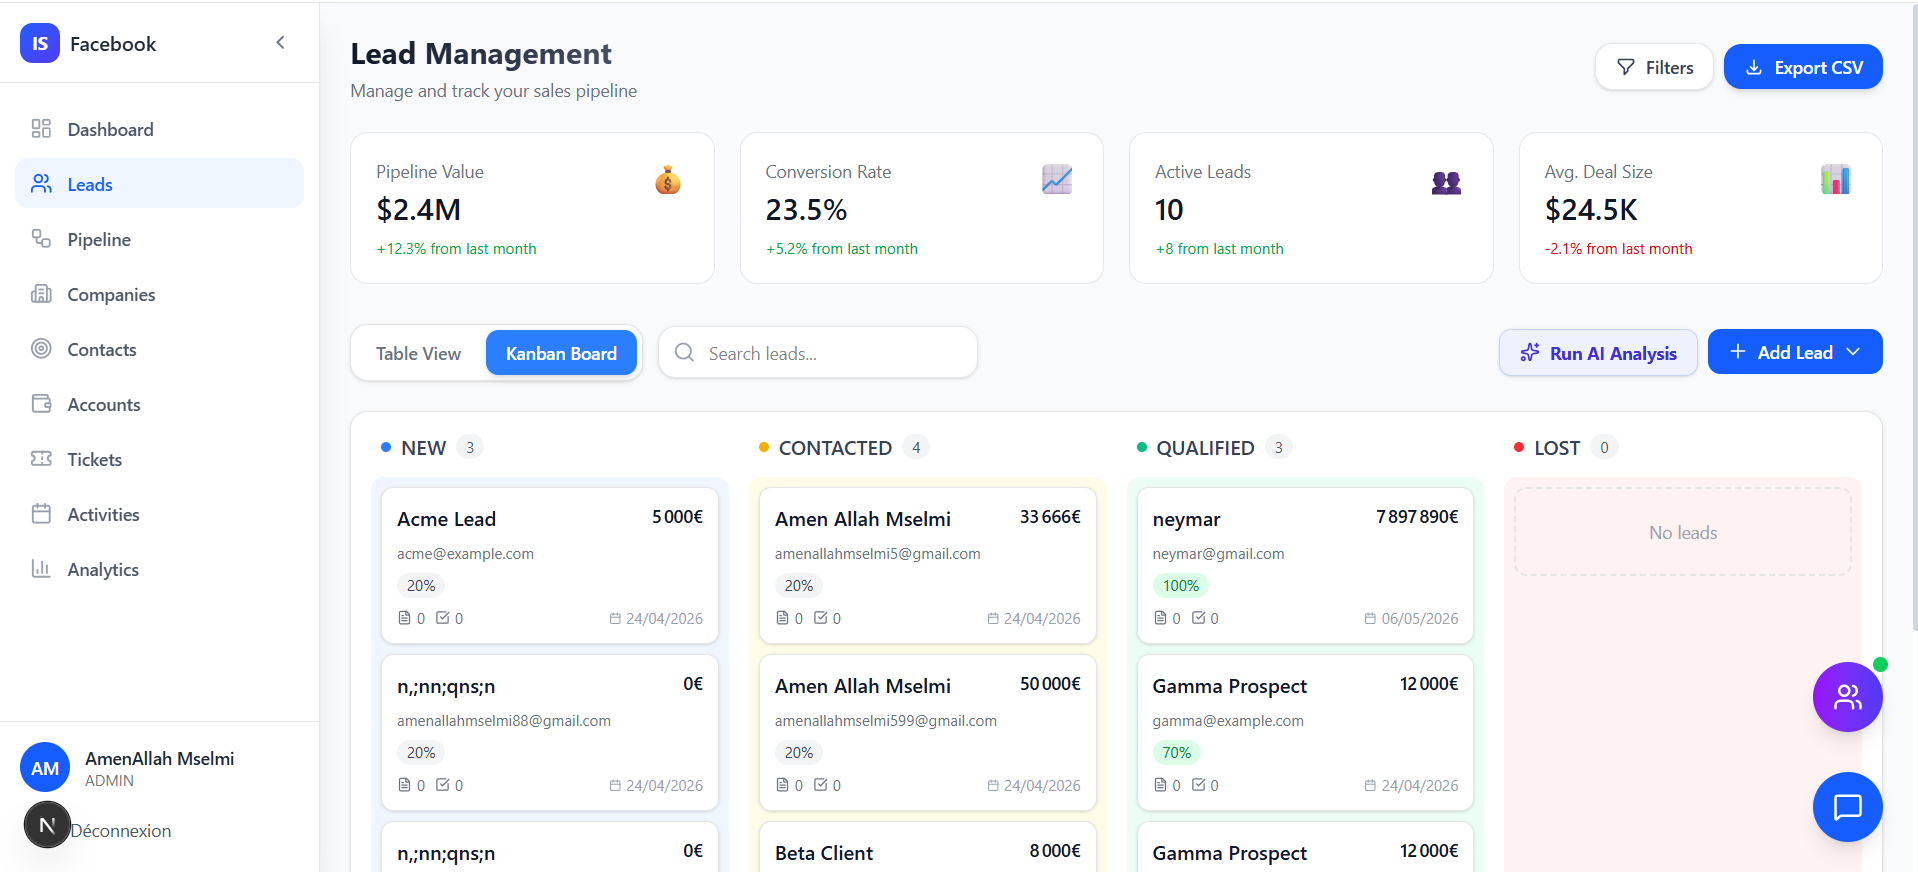
\includegraphics[width=\textwidth,height=0.82\textheight,keepaspectratio]{images/interface_leads.png}
    \caption{Interface gestion des leads}
    \label{fig:leads}
\end{figure}

\subsubsection{Interface détails d'un lead avec scoring IA}
Le score de conversion, qui est calculé par le modèle d'intelligence artificielle (Random Forest), est également visible lorsqu'un administrateur accède à des informations sur un lead. Les informations présentées comprennent la probabilité de conversion, la chaleur du lead (chaud, tiède, froid), ainsi que les principales raisons derrière son score.

\begin{figure}[H]
    \centering
    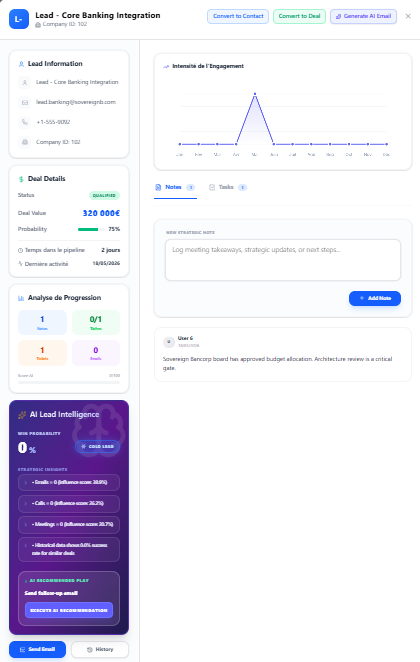
\includegraphics[width=\textwidth,height=0.82\textheight,keepaspectratio]{images/interface_lead_scoring.png}
    \caption{Interface détails d'un lead avec scoring IA}
    \label{fig:lead-scoring}
\end{figure}

\subsubsection{Interface gestion des contacts}
Cette interface liste tous les contacts disponibles dans le CRM. On peut effectuer une recherche, un filtre sur le statut (Active/Inactive), et voir toutes les informations de contact, à savoir leur entreprise correspondante, les courriels et tickets associés.

\begin{figure}[H]
    \centering
    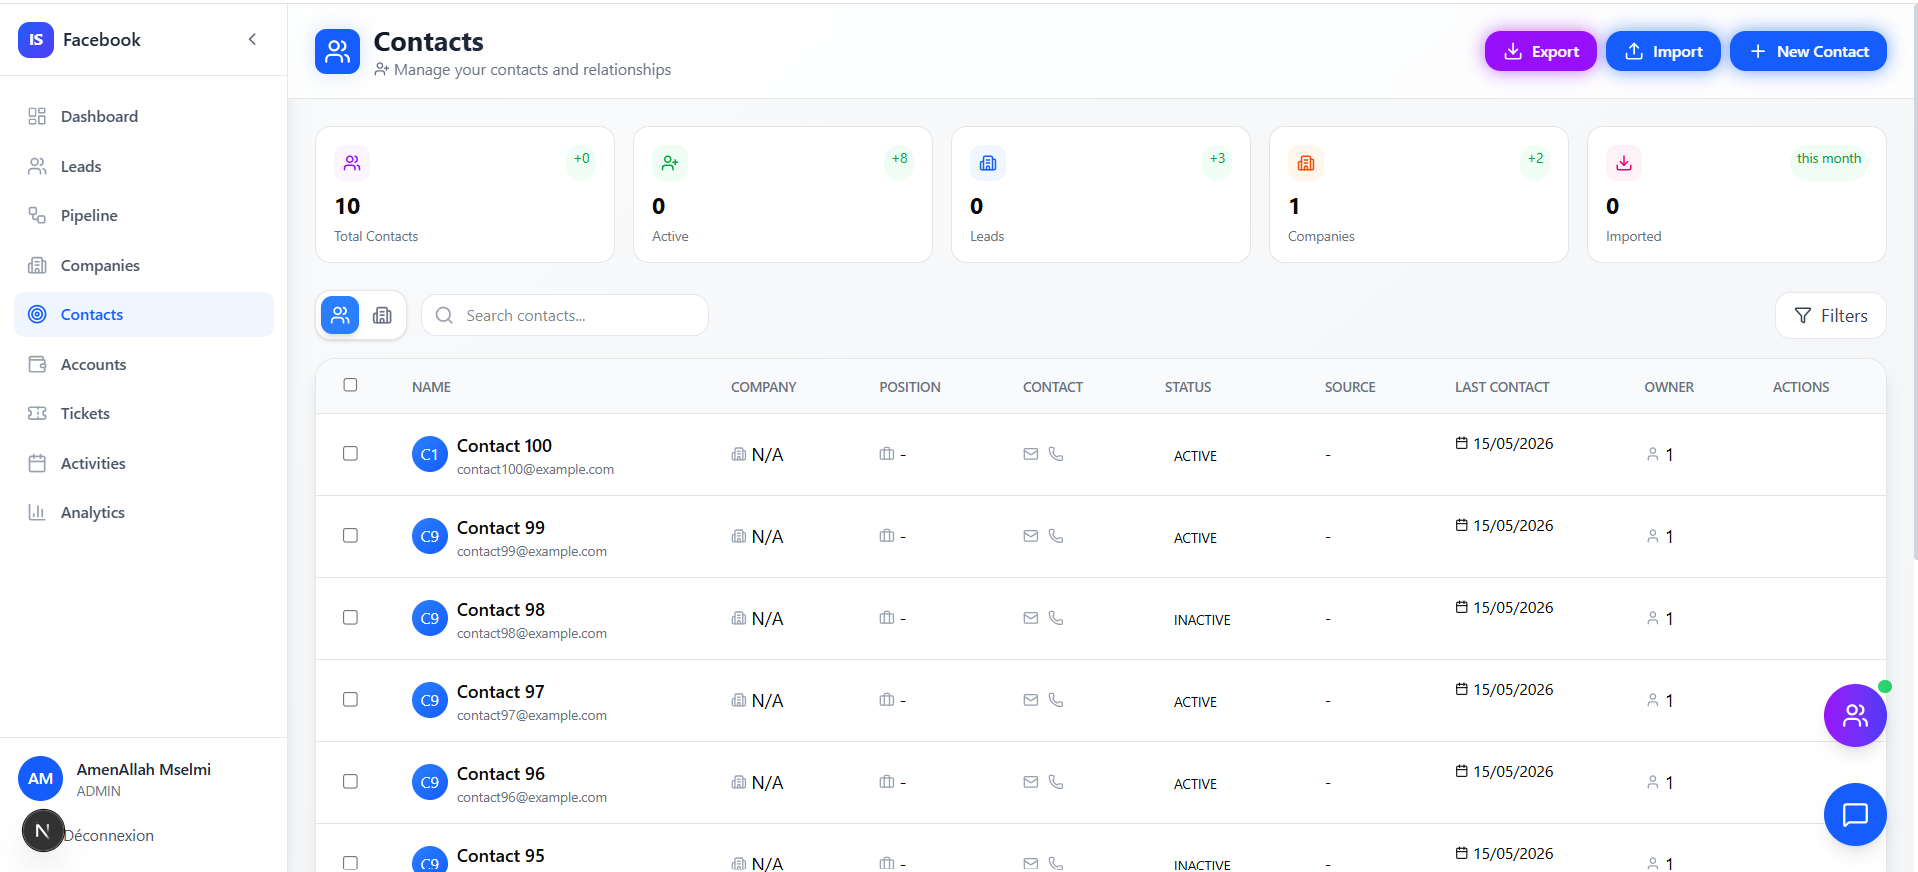
\includegraphics[width=\textwidth,height=0.82\textheight,keepaspectratio]{images/interface_contacts.png}
    \caption{Interface gestion des contacts}
    \label{fig:contacts}
\end{figure}

\subsubsection{Interface gestion des entreprises}
The interface for managing companies shows all the customer companies. Each company is displayed with its name, business sector (Technology, Finance, Healthcare, Education), size (Small, Medium, Large), location, and turnover.

\begin{figure}[H]
    \centering
    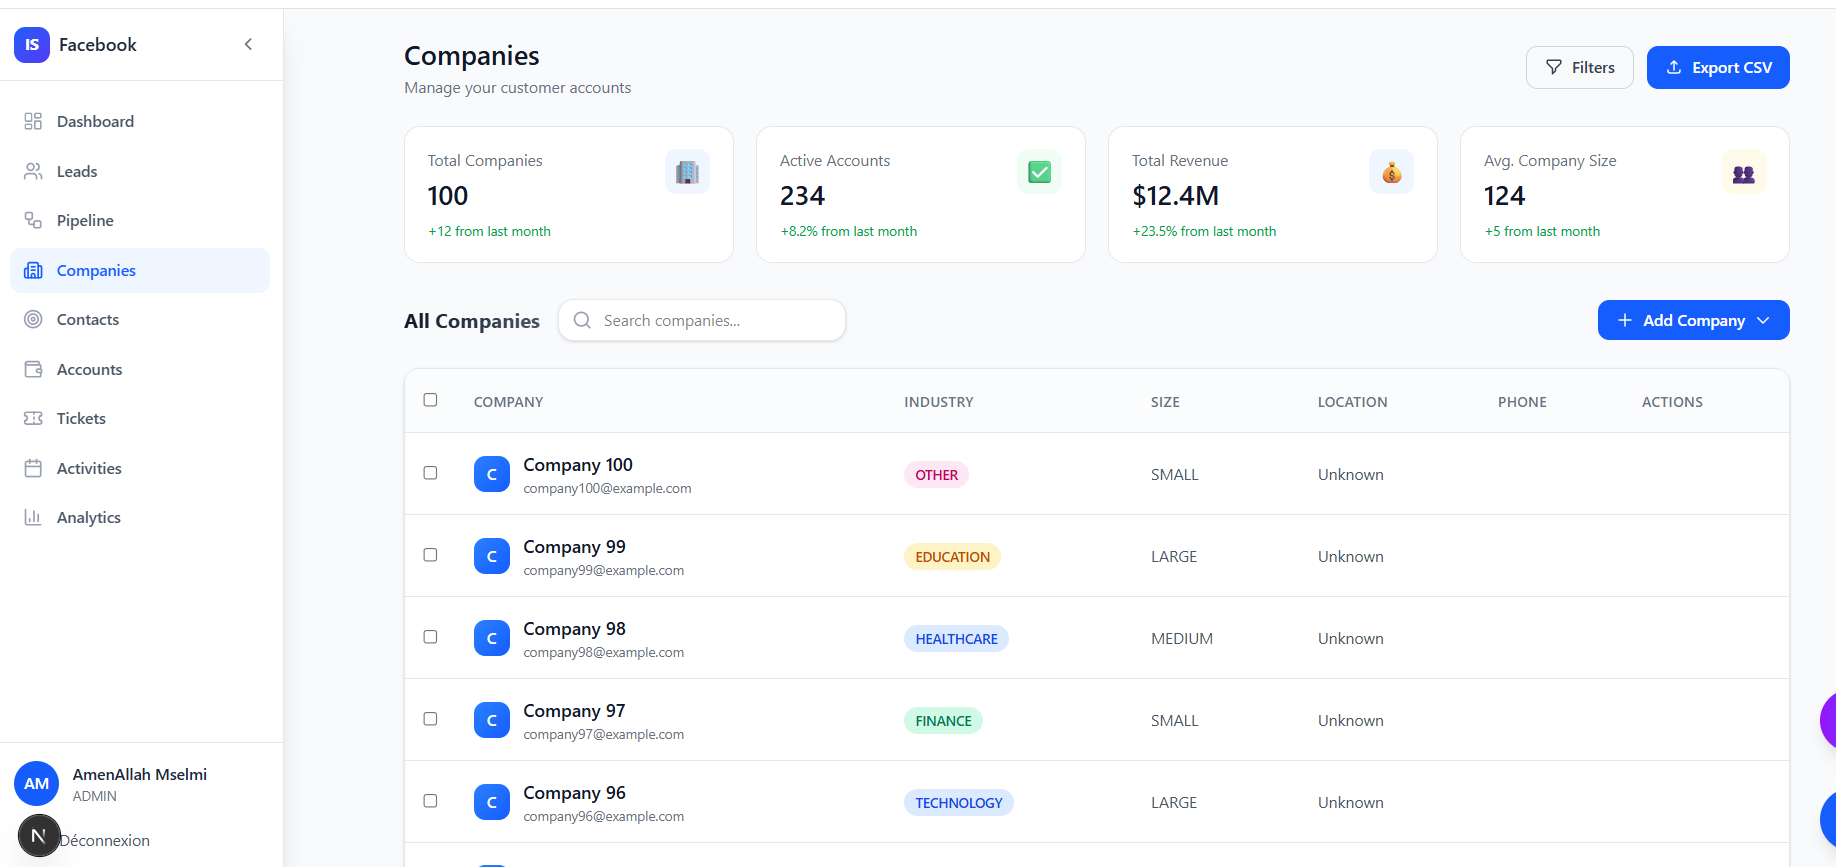
\includegraphics[width=\textwidth,height=0.82\textheight,keepaspectratio]{images/interface_companies.png}
    \caption{Interface gestion des entreprises}
    \label{fig:companies}
\end{figure}

\subsubsection{Interface Pipeline de vente}
La fenêtre de l'interface de pipeline de vente est constituée d'une représentation Kanban de l'affaire qui se divise en plusieurs étapes, notamment Nouvelle, Contactée, Qualifiée, Proposée, Négociée, Gagnée ou Perdue. L'admin peut voir les informations de toutes les affaires dans lesquelles se trouve la société, comme leur valeur, probabilité et date estimée de clôture.

\begin{figure}[H]
    \centering
    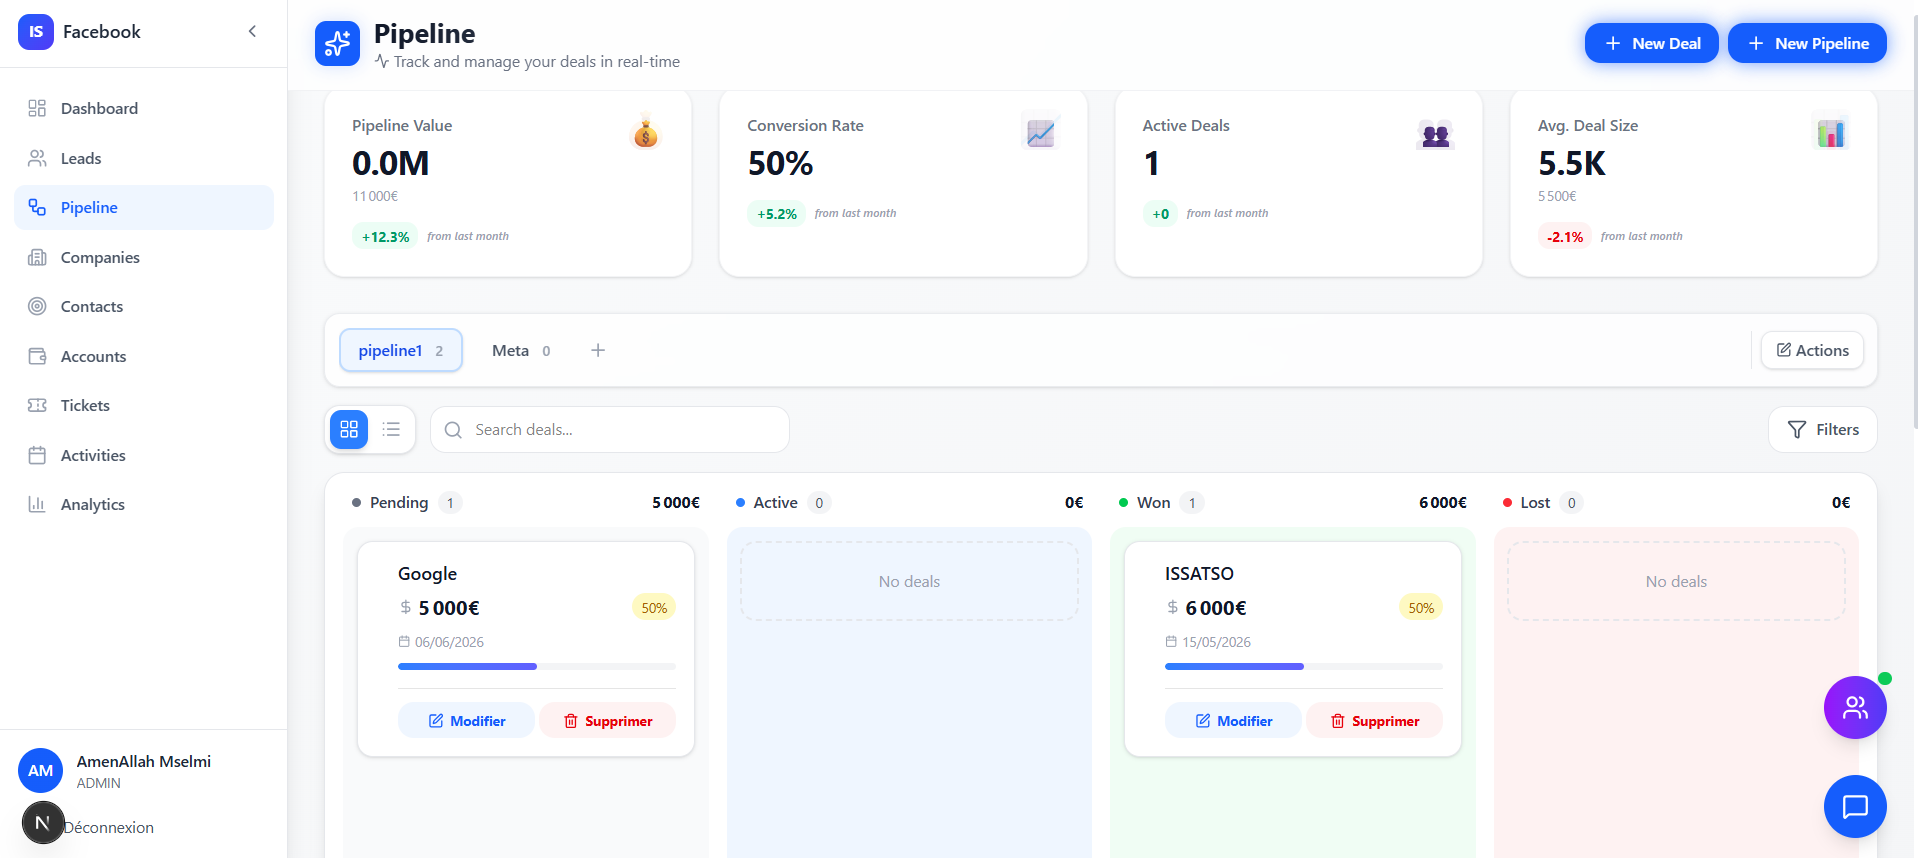
\includegraphics[width=\textwidth,height=0.82\textheight,keepaspectratio]{images/interface_pipeline.png}
    \caption{Interface Pipeline de vente}
    \label{fig:pipeline}
\end{figure}

\subsubsection{Interface gestion des tickets}
La gestion des billets sert à gérer la demande de soutien. La description du billet comprend le nom, la description, l'état (Nouveau, Ouvert, Attendu, Résolu, Fermé) ainsi que la priorité (Basse, Moyenne, Élevée, Critique).

\begin{figure}[H]
    \centering
    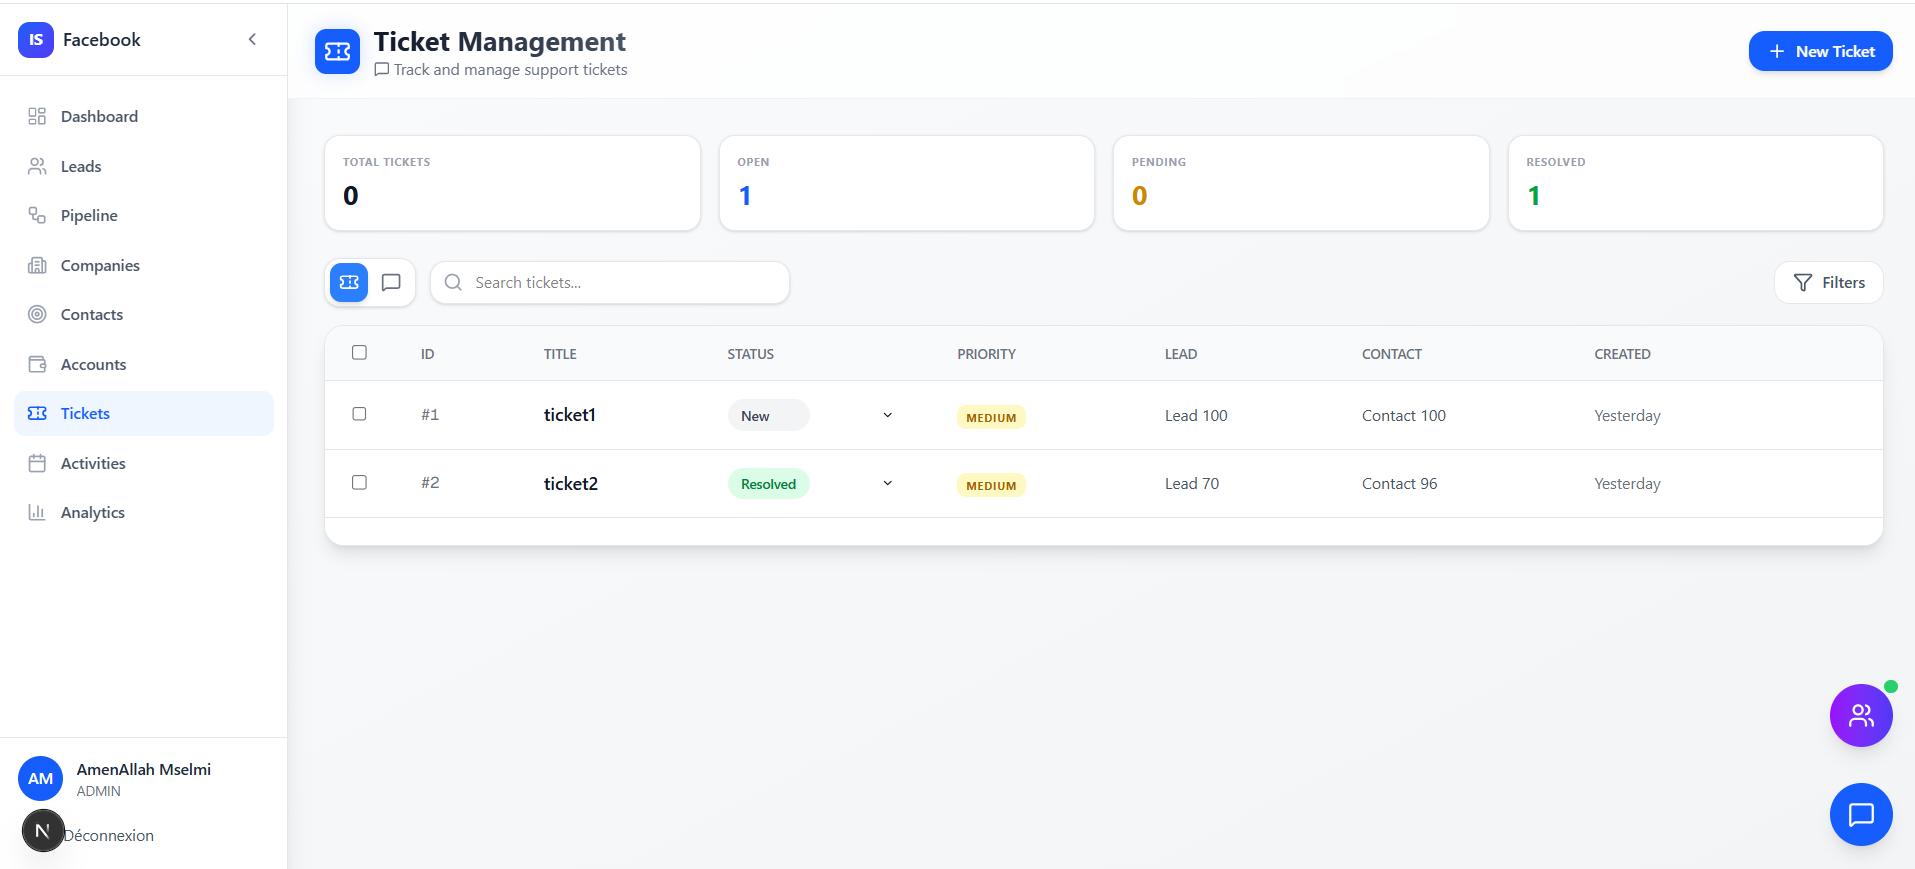
\includegraphics[width=\textwidth,height=0.82\textheight,keepaspectratio]{images/interface_tickets.png}
    \caption{Interface gestion des tickets}
    \label{fig:tickets}
\end{figure}

\subsubsection{Interface Analytics}
Le logiciel analytique permet des visualisations complexes basées sur les données issues du CRM : graphiques de performance de vente, distribution des leads selon l'origine, évolutions temporelles des taux de conversion et productivité des ventes.

\begin{figure}[H]
    \centering
    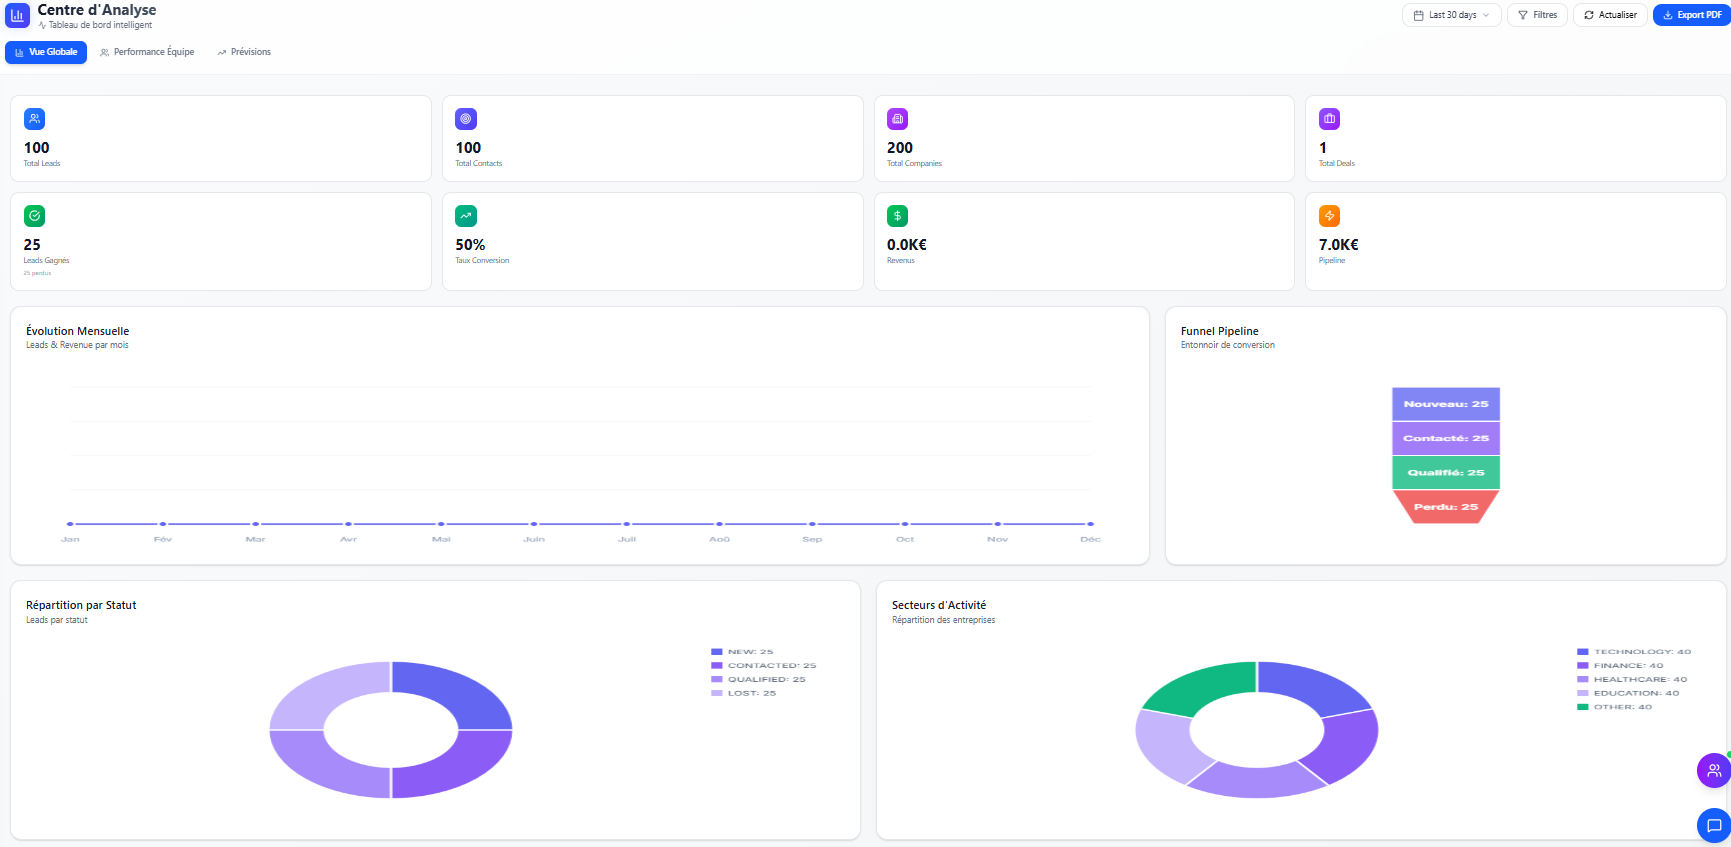
\includegraphics[width=\textwidth,height=0.82\textheight,keepaspectratio]{images/interface_analytics1.png}
    \caption{Interface Analytics - Vue d'ensemble}
    \label{fig:analytics1}
\end{figure}

\begin{figure}[H]
    \centering
    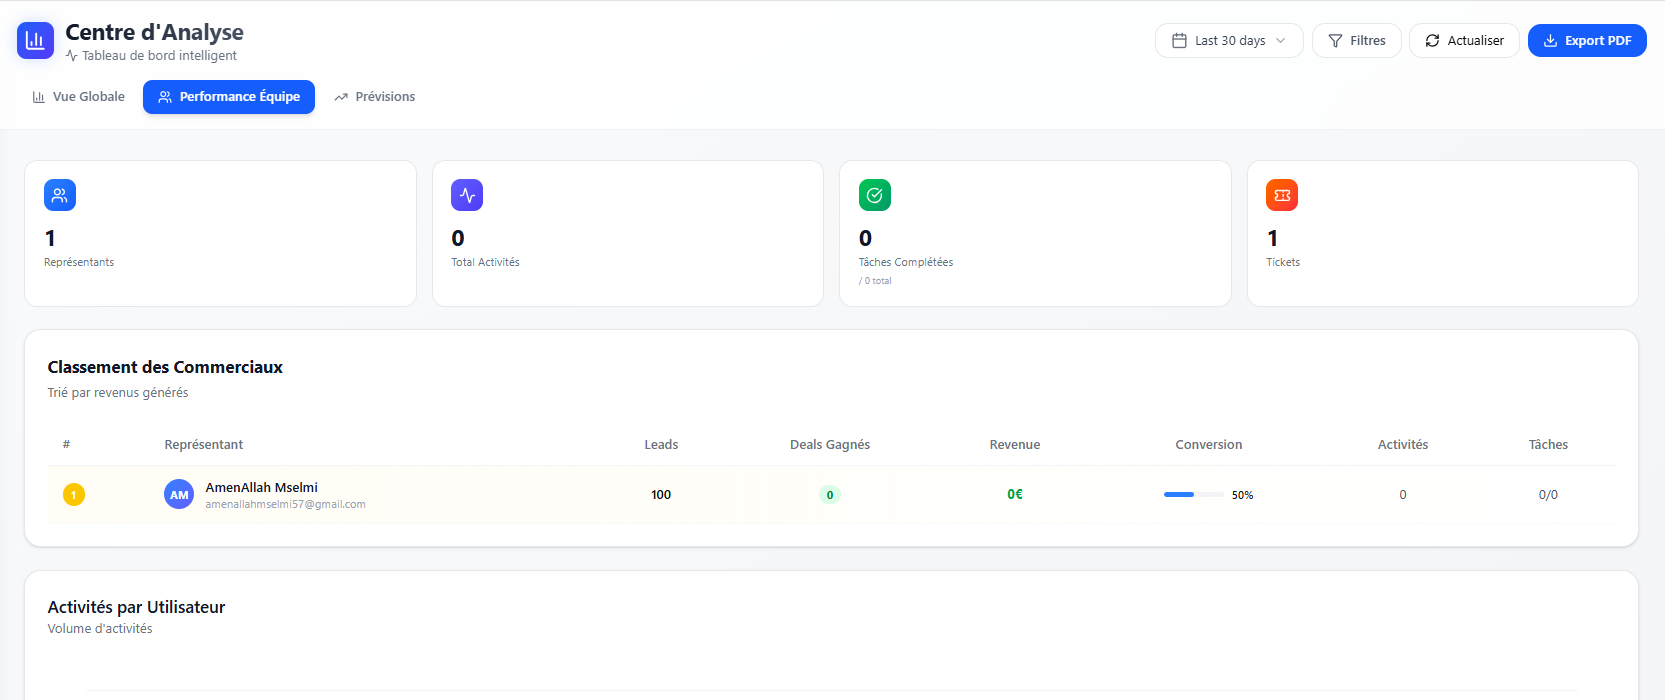
\includegraphics[width=\textwidth,height=0.82\textheight,keepaspectratio]{images/interface_analytics2.png}
    \caption{Interface Analytics - Performance d'équipe}
    \label{fig:analytics2}
\end{figure}

\begin{figure}[H]
    \centering
    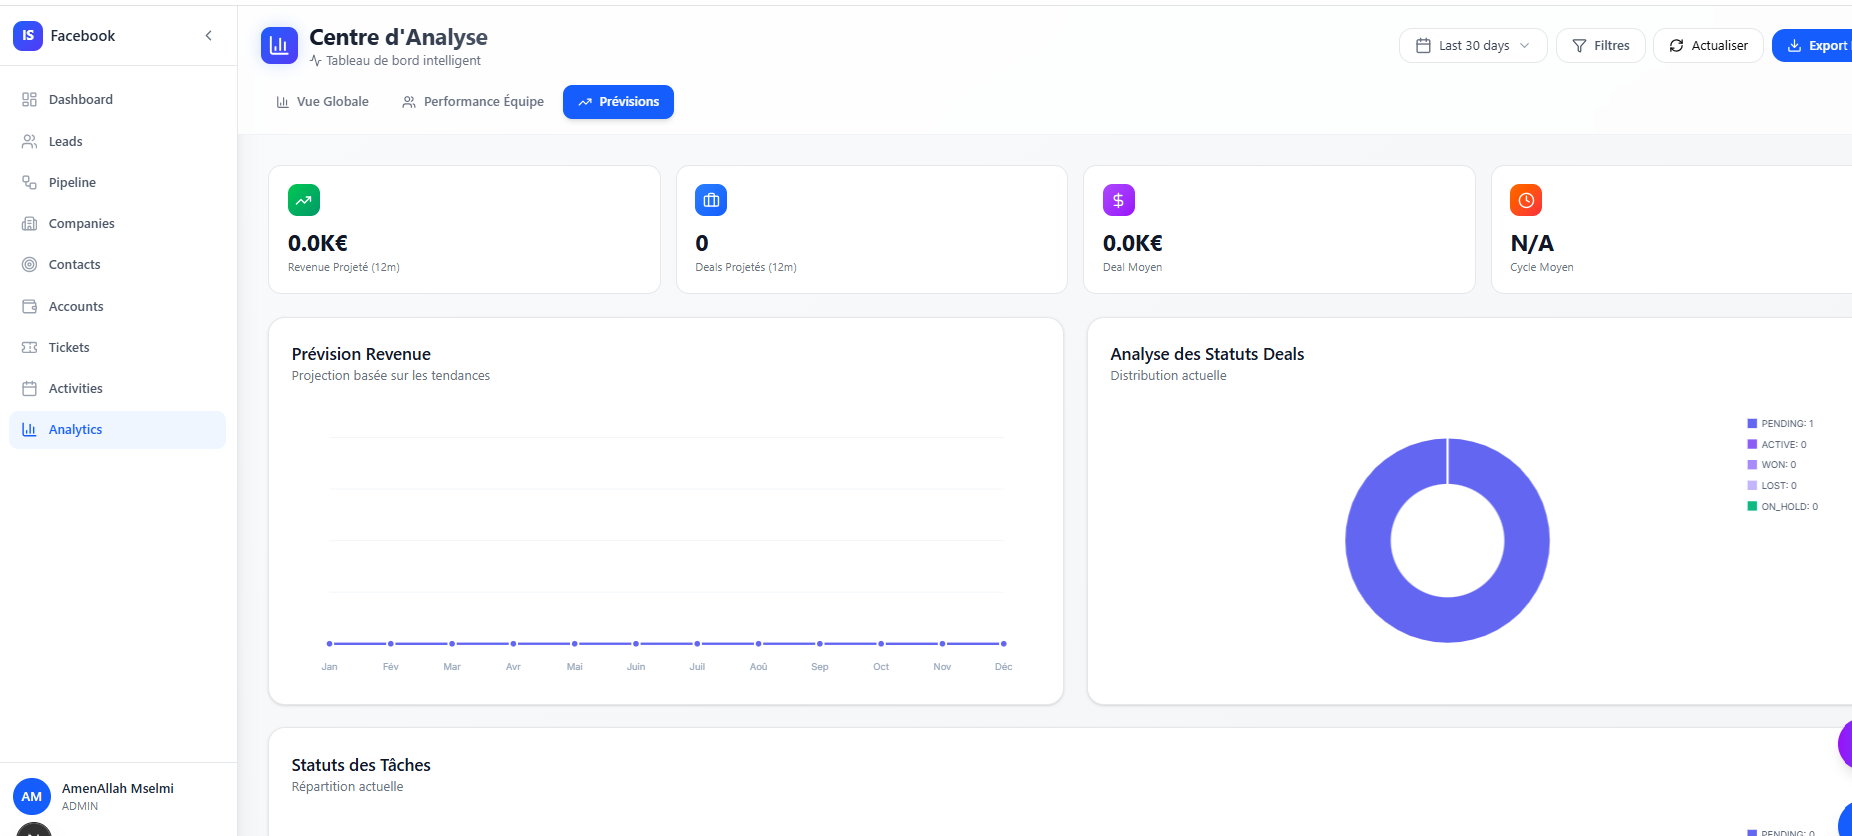
\includegraphics[width=\textwidth,height=0.82\textheight,keepaspectratio]{images/interface_analytics3.png}
    \caption{Interface Analytics - Prévisions}
    \label{fig:analytics3}
\end{figure}

\subsubsection{Interface gestion des comptes}
Il y a une interface pour la gestion des comptes où l'administrateur peut ajouter des comptes aux Sales Reps, modifier les paramètres de ces comptes, et activer ou désactiver ces comptes.

\begin{figure}[H]
    \centering
    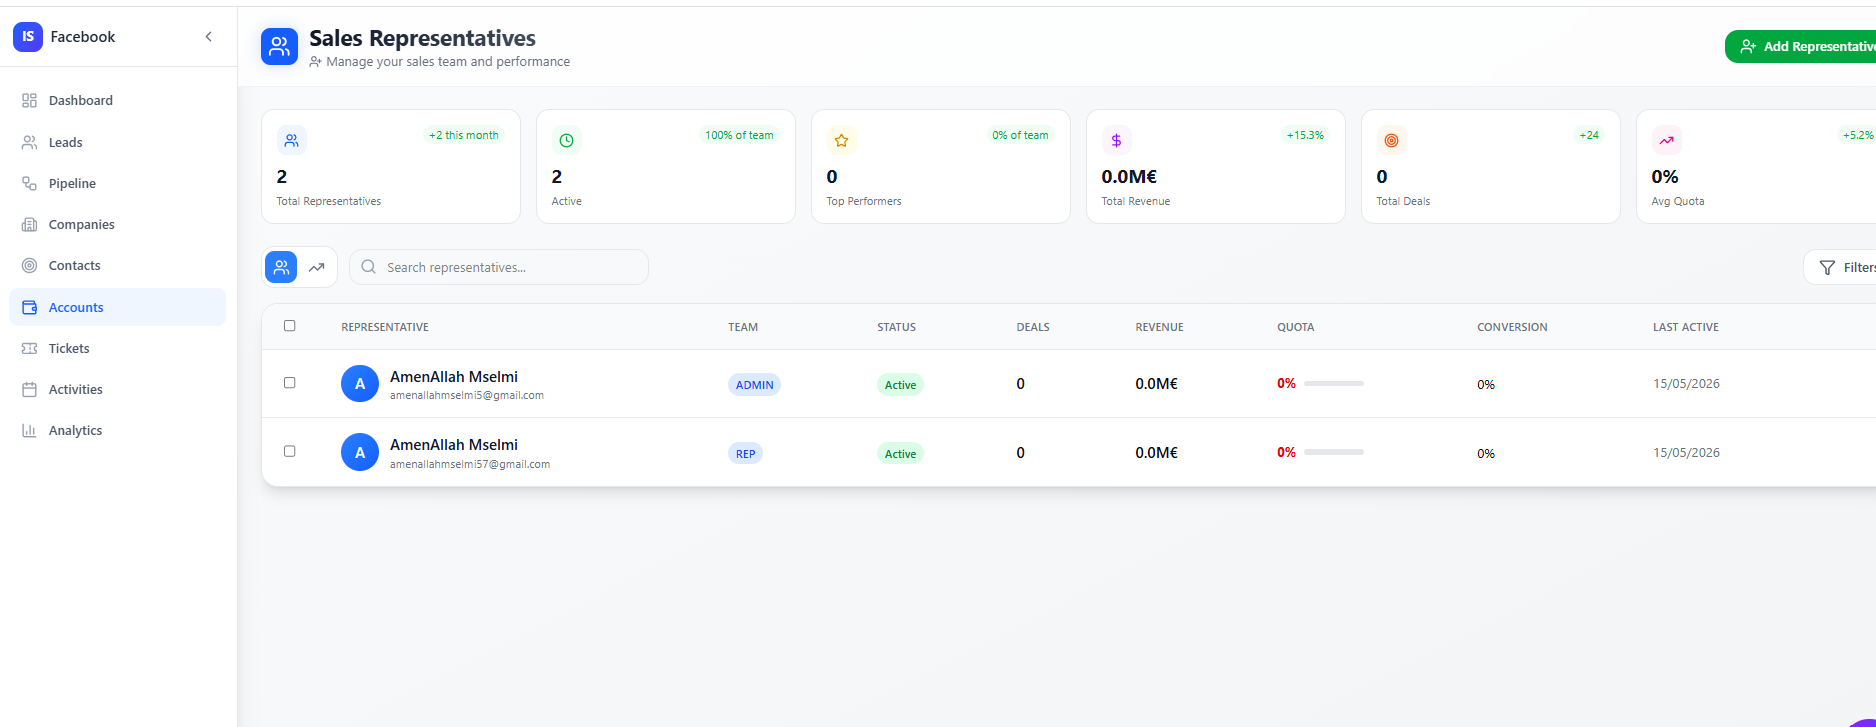
\includegraphics[width=\textwidth,height=0.82\textheight,keepaspectratio]{images/interface_accounts.png}
    \caption{Interface gestion des comptes utilisateurs}
    \label{fig:accounts}
\end{figure}

\subsection{Partie Sales Representative (Rep)}

\subsubsection{Interface tableau de bord Rep}
Dashboard du Sales Representative indique ses propres KPIs : lead assignés, deals actifs, les tâches qui lui sont attribuées et des tickets qu'il possède. Le design donne une vue d'ensemble de son travail commercial quotidien.

\begin{figure}[H]
    \centering
    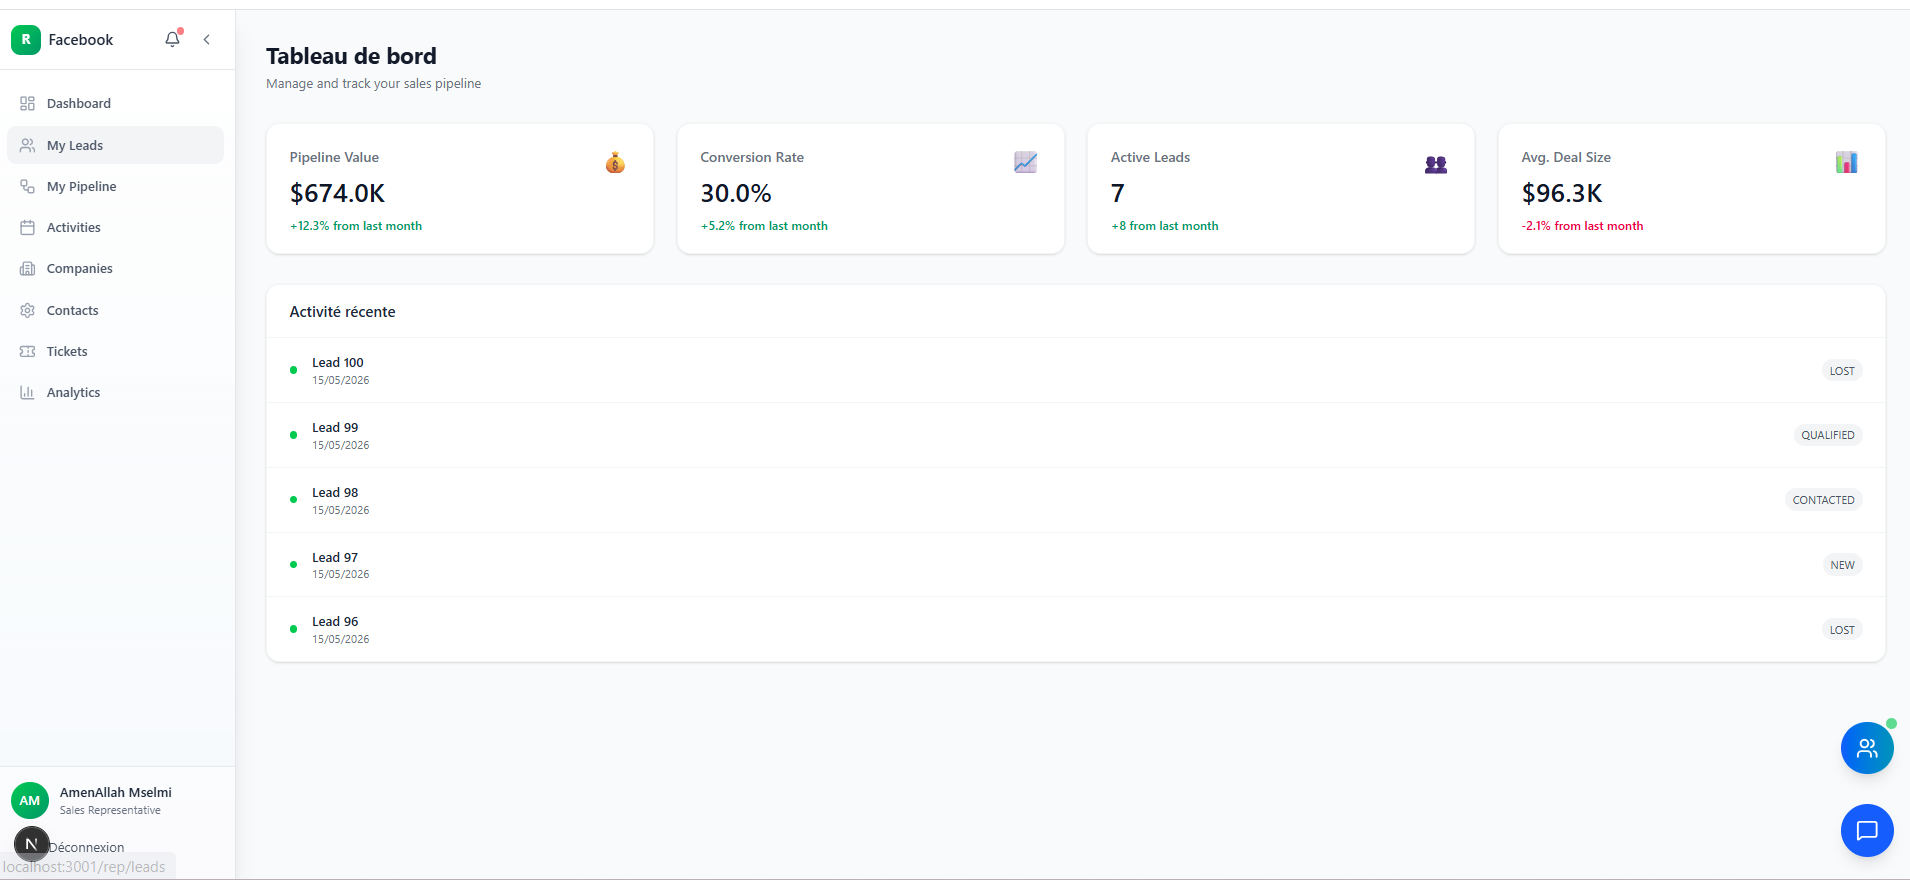
\includegraphics[width=\textwidth,height=0.82\textheight,keepaspectratio]{images/interface_dashboard_rep.png}
    \caption{Interface tableau de bord Sales Representative}
    \label{fig:dashboard-rep}
\end{figure}

\subsubsection{Interfaces du Rep -- Leads, Contacts et Pipeline}
Le Sales Representative a des interfaces qui sont comparables à celles de l'Admin mais uniquement sur ses propres données. Il peut gérer ses leads, contacts et pipeline personnels, en ayant la capacité d'ajouter des commentaires, créer des tâches et envoyer des messages électroniques.

\begin{figure}[H]
    \centering
    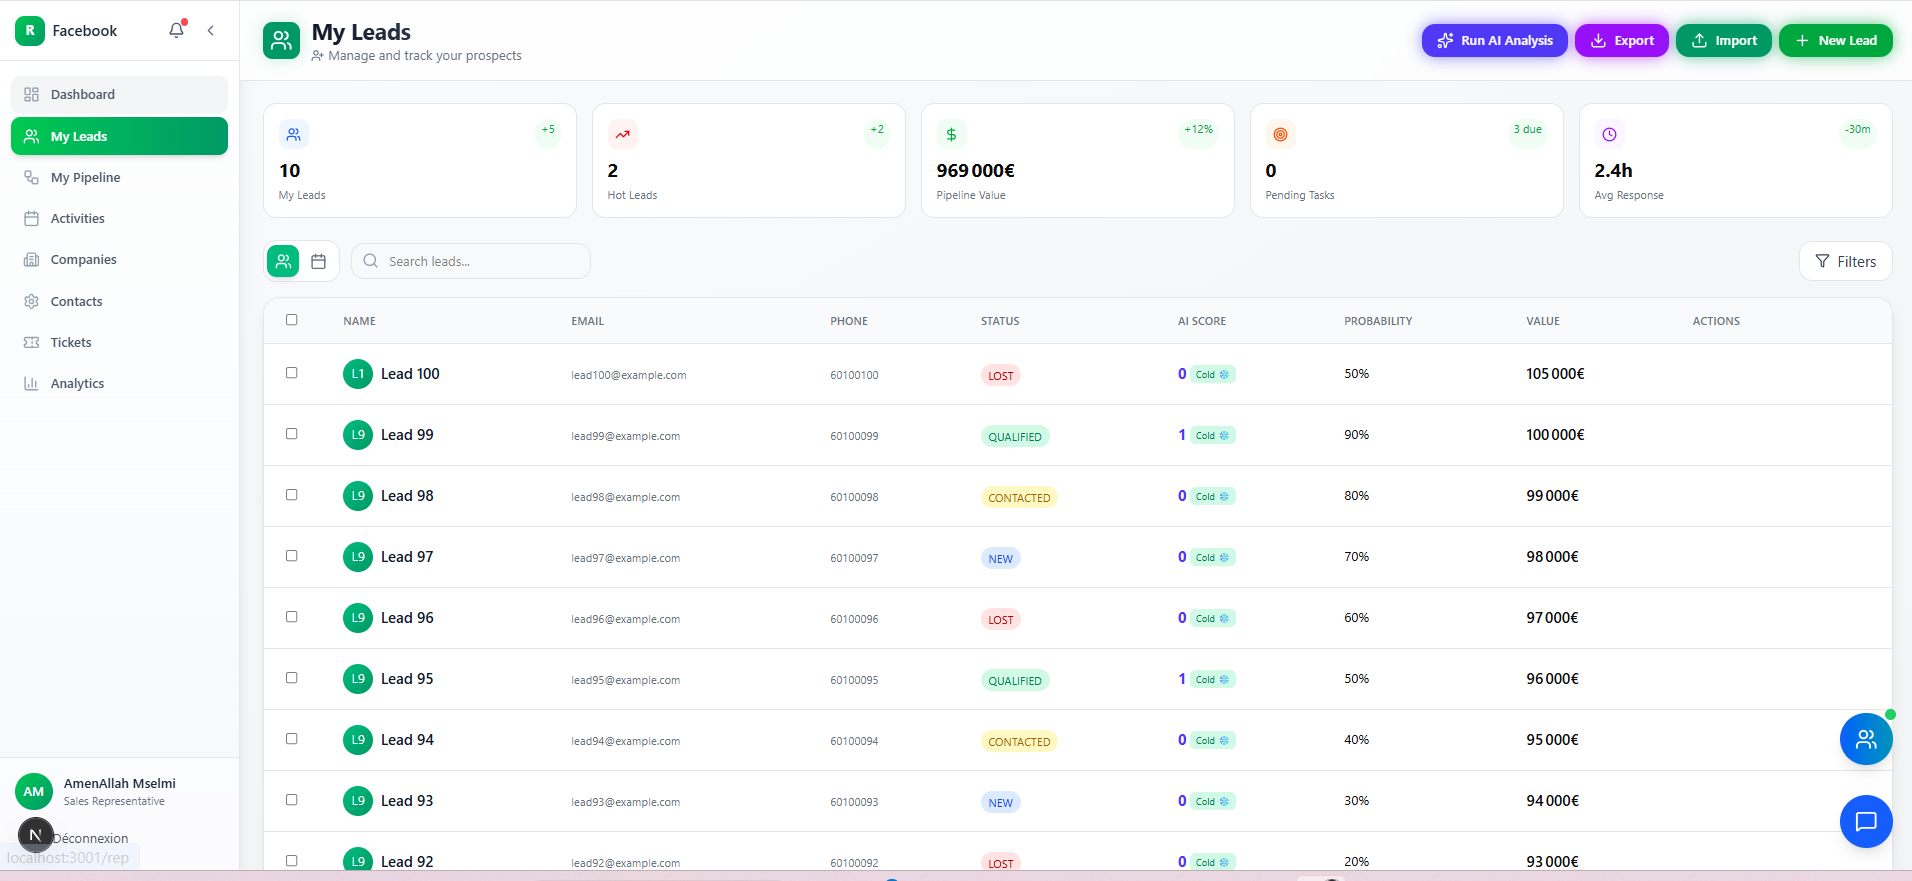
\includegraphics[width=\textwidth,height=0.82\textheight,keepaspectratio]{images/interface_rep_leads.png}
    \caption{Interface leads du Sales Representative}
    \label{fig:rep-leads}
\end{figure}

\subsection{Fonctionnalités transversales}

\subsubsection{Interface de Chat en temps réel}
Le module de chat est constitué d'une interface qui facilite la communication en temps réel entre les utilisateurs via WebSocket (Socket.io). Il permet aux utilisateurs d'échanger des messages, d'avoir des conversations privées ou de groupe, et d'être notifiés lorsqu'ils reçoivent un nouveau message.

\begin{figure}[H]
    \centering
    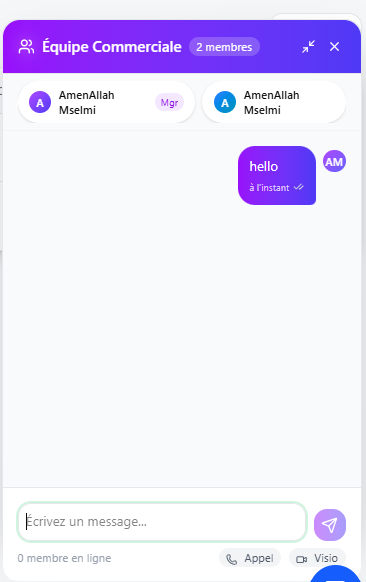
\includegraphics[width=\textwidth,height=0.82\textheight,keepaspectratio]{images/interface_chat.png}
    \caption{Interface de Chat en temps réel}
    \label{fig:chat}
\end{figure}

\subsubsection{Interface d'import CSV}
L'assistant d'import des données CSV donne un assistant étape par étape, permettant la facilité d'importer de nombreuses données de leads ou de contacts d'un fichier CSV. Les utilisateurs peuvent mapper les colonnes du fichier avec les champs CRM et importer les données.

\begin{figure}[H]
    \centering
    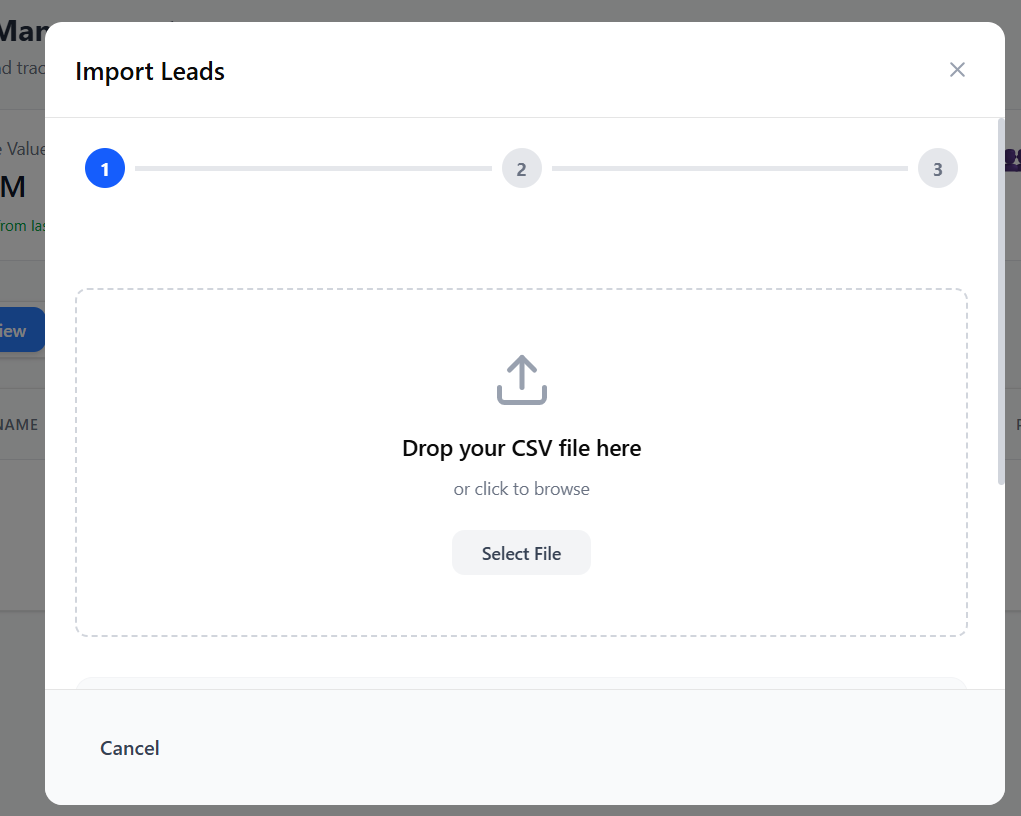
\includegraphics[width=\textwidth,height=0.82\textheight,keepaspectratio]{images/interface_csv_import1.png}
    \caption{Interface d'import CSV - Étape 1}
    \label{fig:csv-import1}
\end{figure}

\begin{figure}[H]
    \centering
    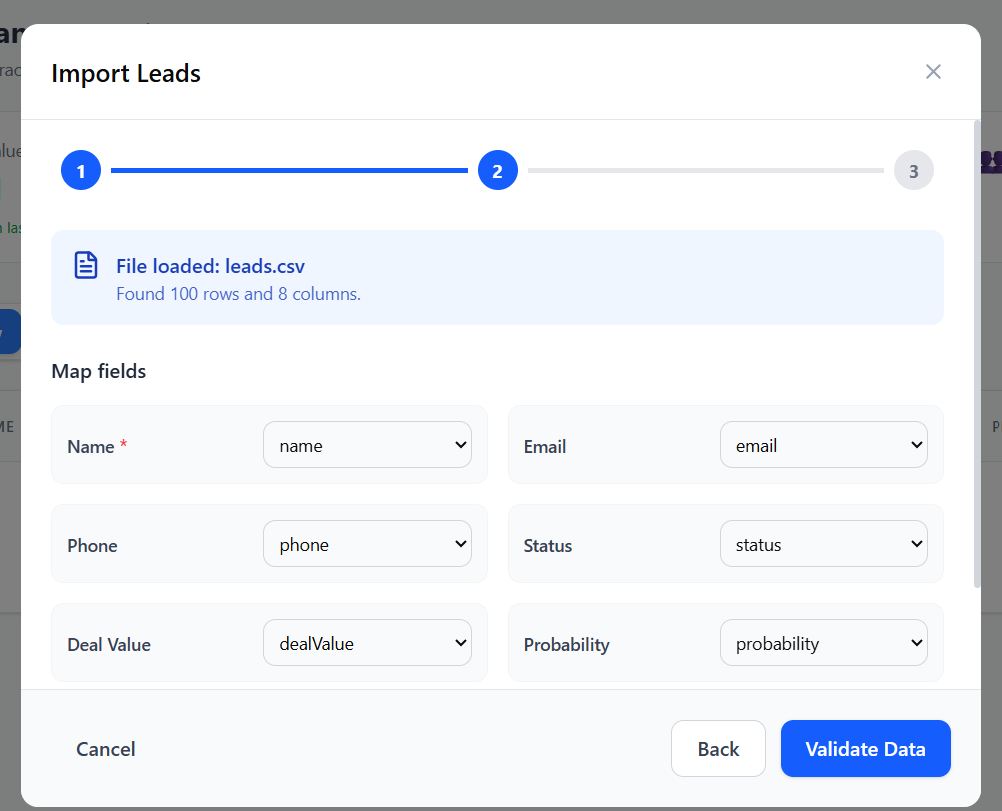
\includegraphics[width=\textwidth,height=0.82\textheight,keepaspectratio]{images/interface_csv_import2.png}
    \caption{Interface d'import CSV - Étape 2}
    \label{fig:csv-import2}
\end{figure}

\begin{figure}[H]
    \centering
    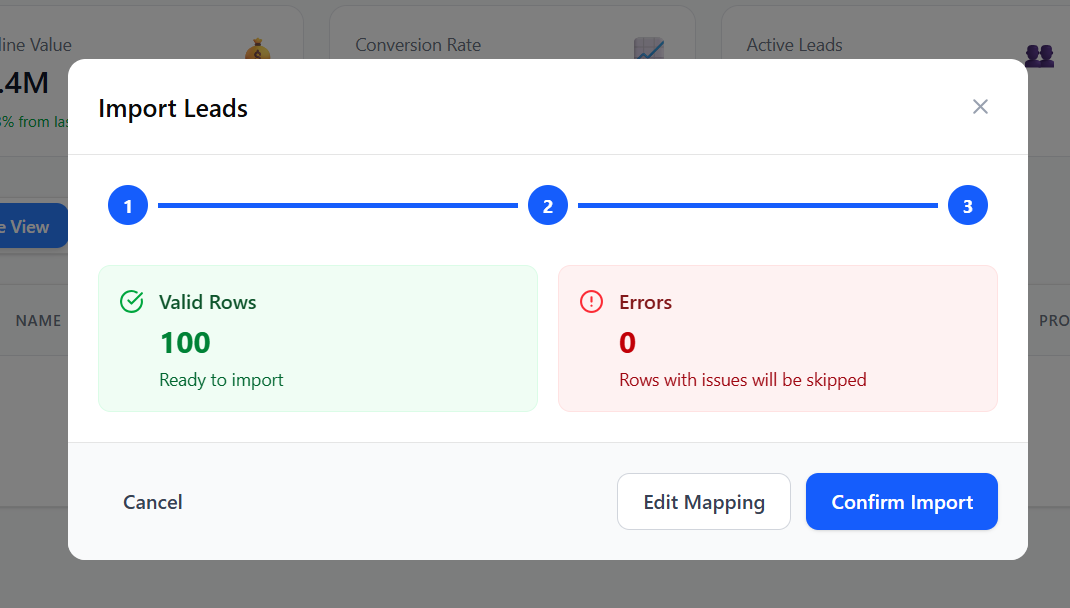
\includegraphics[width=\textwidth,height=0.82\textheight,keepaspectratio]{images/interface_csv_import3.png}
    \caption{Interface d'import CSV - Étape 3}
    \label{fig:csv-import3}
\end{figure}

\subsubsection{Interface de génération d'e-mails par IA}
Avec l'intégration de l'API Gemini de Google, il est possible de générer des e-mails personnalisés à destination de ses prospects et contacts. Une intelligence artificielle propose un contenu qui convient au contexte du prospect et à son stade dans le tunnel de conversion.

\begin{figure}[H]
    \centering
    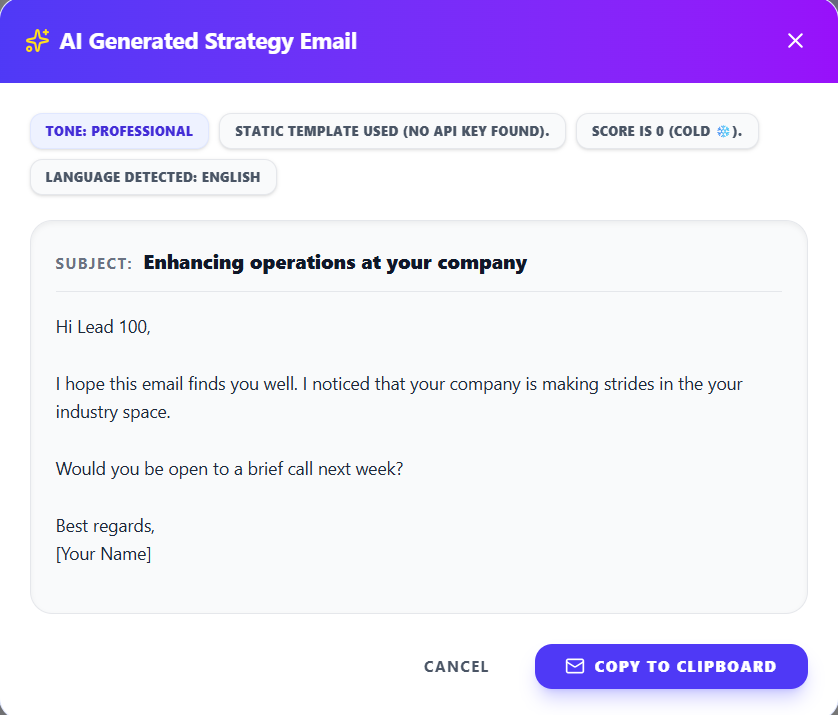
\includegraphics[width=\textwidth,height=0.82\textheight,keepaspectratio]{images/interface_ai_email.png}
    \caption{Interface de génération d'e-mails par IA}
    \label{fig:ai-email}
\end{figure}

\subsubsection{Assistant conversationnel (Chatbot) intelligent avec RAG}
Afin d'accompagner les commerciaux et managers dans leurs activités quotidiennes, nous avons développé un assistant virtuel flottant (Chatbot). Pour que cet assistant puisse répondre intelligemment et éviter les réponses génériques ou "hors-sujet", nous avons implémenté l'architecture \textbf{RAG} (Retrieval-Augmented Generation) au sein de la plateforme.

Lorsqu'un utilisateur pose une question (par exemple : \textit{"Combien avons-nous de leads qualifiés ?"} ou \textit{"Quels sont nos deals gagnés récents ?"}), le backend NestJS interroge de manière dynamique MySQL à travers Prisma pour collecter un contexte structuré (statistiques de ventes, pipeline, leads récents et tâches urgentes). Ce contexte est ensuite formaté et transmis de façon sécurisée à l'API Google Gemini (\textit{gemini-2.5-flash}) qui rédige une réponse précise, en français, et basée exclusivement sur les données réelles du CRM.

\begin{figure}[H]
    \centering
    % % \includegraphics[width=0.45\textwidth]{images/interface_chatbot.png}
    \caption{Interface de l'assistant conversationnel (Chatbot) RAG (Image manquante)}
    \label{fig:chatbot}
\end{figure}

\subsubsection{Tableau de bord Power BI}
En complément des analytiques intégrées, nous avons développé un tableau de bord Power BI connecté à la base de données MySQL. Ce dashboard offre des visualisations interactives avancées pour l'analyse des tendances de vente, la performance des commerciaux et les prévisions de revenus.

\begin{figure}[H]
    \centering
    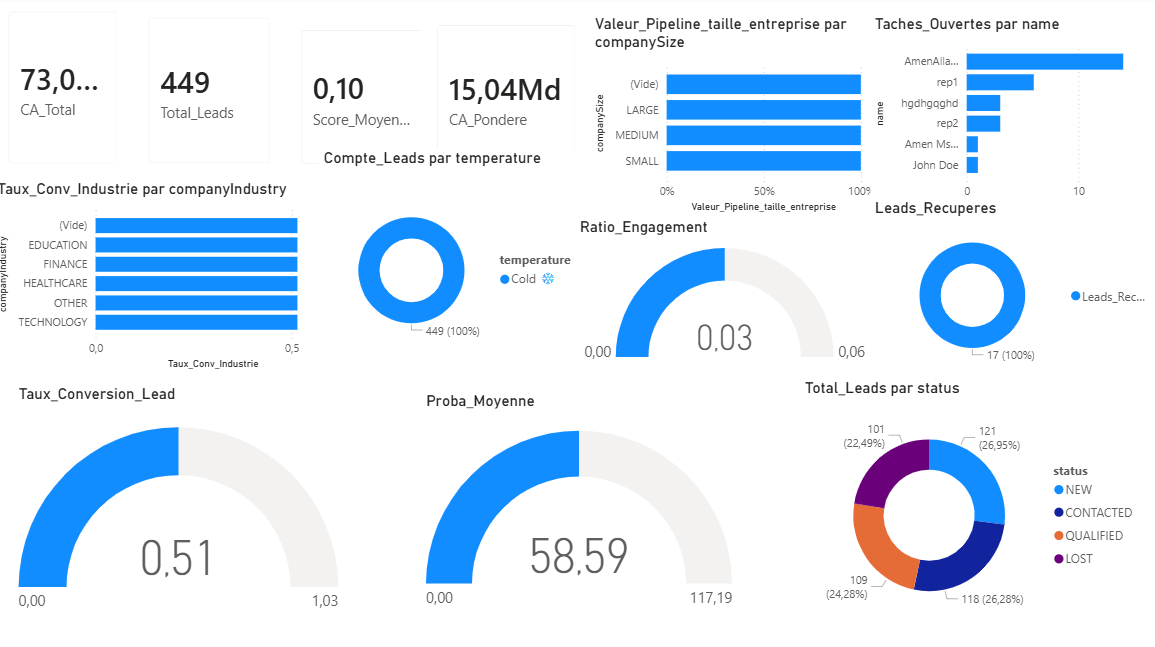
\includegraphics[width=\textwidth,height=0.82\textheight,keepaspectratio]{images/interface_powerbi1.png}
    \caption{Résumé exécutif Power BI}
    \label{fig:powerbi1}
\end{figure}

\begin{figure}[H]
    \centering
    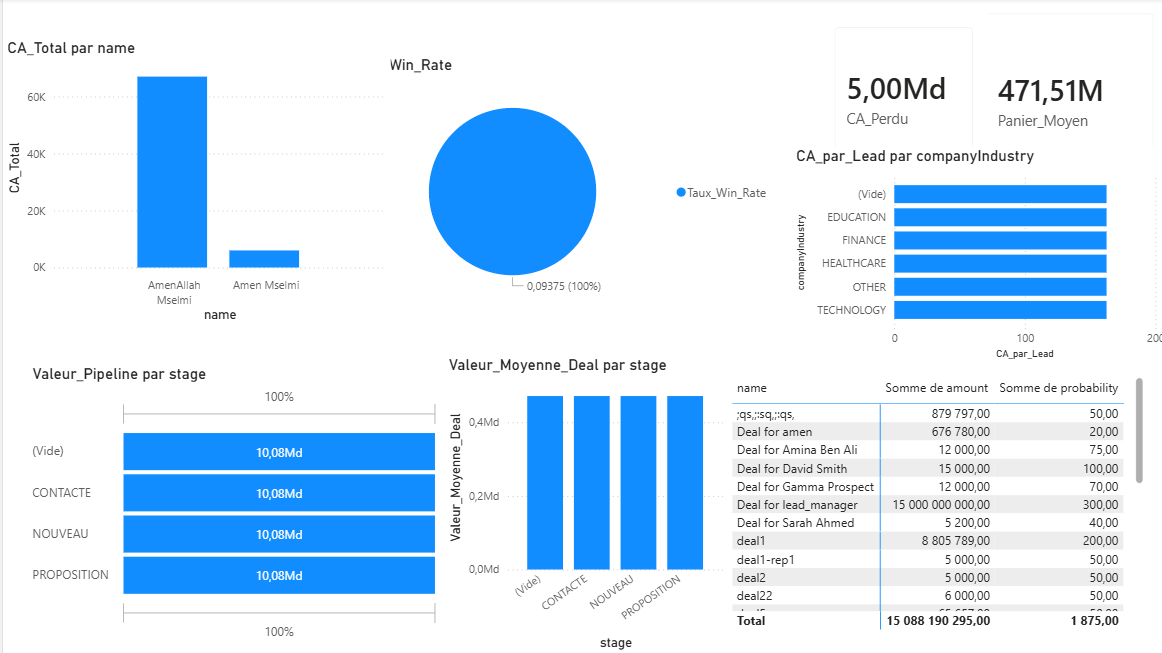
\includegraphics[width=\textwidth,height=0.82\textheight,keepaspectratio]{images/interface_powerbi2.png}
    \caption{Pipeline de ventes Power BI}
    \label{fig:powerbi2}
\end{figure}

\begin{figure}[H]
    \centering
    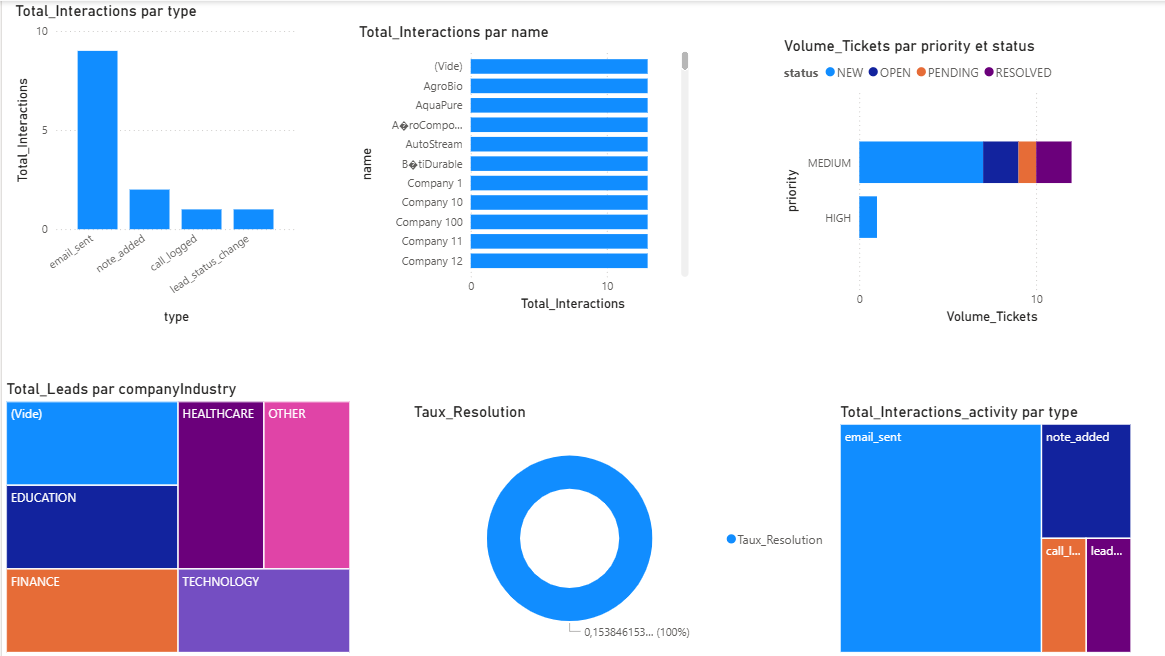
\includegraphics[width=\textwidth,height=0.82\textheight,keepaspectratio]{images/interface_powerbi3.png}
    \caption{Engagement client Power BI}
    \label{fig:powerbi3}
\end{figure}

%% ============================================================
%%  CONCLUSION
%% ============================================================
\section*{Conclusion}

Dans la phase de réalisation, nous avons utilisé des environnements techniques et logiciels spécifiques pour développer notre plateforme CRM avec scoring de leads par intelligence artificielle. Nous avons présenté notre application en illustrant ses fonctionnalités principales à travers les interfaces développées. L'architecture microservices adoptée, combinée à la conteneurisation Docker et à l'orchestration Kubernetes, assure la scalabilité et la maintenabilité de notre solution. Le pipeline CI/CD via GitHub Actions garantit un déploiement automatisé et fiable. En conclusion, nous sommes satisfaits du résultat obtenu et nous envisageons des perspectives d'amélioration pour les prochaines versions.
